
\documentclass{aa}  

\usepackage{graphicx}
\usepackage{float}
\usepackage{subcaption}
\usepackage{mwe}
\usepackage{txfonts}
\usepackage{hyperref}
\hypersetup{
    colorlinks=true,
    linkcolor=black,
    filecolor=black,  
    citecolor=black,
    urlcolor=black,
    pdftitle={Yukawa's meson theory of Nuclear Forces},
    pdfpagemode=FullScreen,
    pdfauthor={Cano Jones, Alejandro},
    pdfcreator={Cano Jones, Alejandro},
    pdfnewwindow=true,
}


\begin{document} 


   \title{Photometric catalog of NGC 6793}

   \subtitle{Observational Astrophysics final project}

   \author{A. Cano Jones\inst{1} }

   \institute{Universidad de Zaragoza, \href{https://estudios.unizar.es/estudio/ver?id=719}{Máster Universitario en Física del Universo}\\
   e-mail: \href{mailto:728137@unizar.es}{728137@unizar.es}
             }

   \date{Dated: \today}
 
  \abstract
  % context heading (optional)
  % {} leave it empty if necessary  
   {}
  % aims heading (mandatory)
   {...}
  % methods heading (mandatory)
   {...}
  % results heading (mandatory)
   {..}
  % conclusions heading (optional), leave it empty if necessary 
   {}
   

   \keywords{Methods: data analysis -- Techniques: photometric
 -- Catalogs -- (Galaxy:) open clusters and associations: individual: NGC 6793
               }

   \maketitle
    \section{Introduction}\label{sec: Introduction}
    Open clusters are groups of young stars (few million to a few hundred million years) which number ranges from tens to a few thousand stars formed from the same molecular cloud that are loosely  gravitationally bound together. 
    Stars from the same clusters have similar composition and ages, where the main difference comes from their masses, reason why they serve as valuable laboratories for studying stellar evolution, since comparing two stars from the same cluster most of the parameters remain unchanged. Notable examples of open clusters include the Pleiades, Hyades or the Alpha Persei Cluster.

    The NGC 6793 open cluster was discovered (\cite{Seligman_2018}) by William Herschel the night of the 18Th of July of 1789, and was later cataloged by John Louis Emil Dreyer in his \textit{New General Catalogue of Nebulae and Clusters of Stars} (abbreviated NGC) with the simple description of ``a cluster, poor, a little compressed''. Is located in the Vulpecula constellation, close to the celestial equator with (\cite{SIMBAD}) celestial coordinates (J2000 equinox) 19h 23m 13s (RA) \& +22° 08’ 27” (DEC); its angular size is $27.2\times27.2$ arcmin and a parallax of $1.6672\pm 0.0021$ mas. 

    Throughout this paper, the process by which a photometric catalogue of the NGC 6793 open cluster was obtained will be detailed; from on-site observations made at the main telescope in Galáctica (section \ref{sec: Photometric data collection}), passing through the reduction and calibration of the obtained photometric images (section \ref{sec: Image reduction and calibration}), up to the building of the catalog of stars present in the photometric images over four filters (section \ref{sec: Photometric catalogs}), from which some results will be extracted (section \ref{sec: Results}).
    %%%%%%%%%%%%%%%%%%%%%%%%%%%%%%%%%%%%%%%%%%%%%%%%%%%%%%%%%%%%%%%%%%%%%%%%%%%%%%%%%%%%%%%
    \section{Photometric data collection}\label{sec: Photometric data collection}
    The photometric data collection was performed the night of the 20Th of April, 2023 at 02:41 LM, a night without moon and (at the time of observations) clear skies; using the 80cm (f/7) telescope at the Centre for the Dissemination and Practice of Astronomy: Galactica (Teruel, Spain). The telescope's  camera has a pixel of 0.5" and a field of view of $19\times19$ arcmin$^2$, ensuring that the whole cluster fits in one image. Previous work was made to ensure the visibility of the cluster using the online app \textit{Object Visivility-STARALT} (\cite{STARALT}) and estimates of the exposure times using the online app \textit{CAMELOT2 SNR calculator} (\cite{EXP_Calculator}).
    \begin{figure}[H]
      \centering
      \subfloat[][rSDSS]{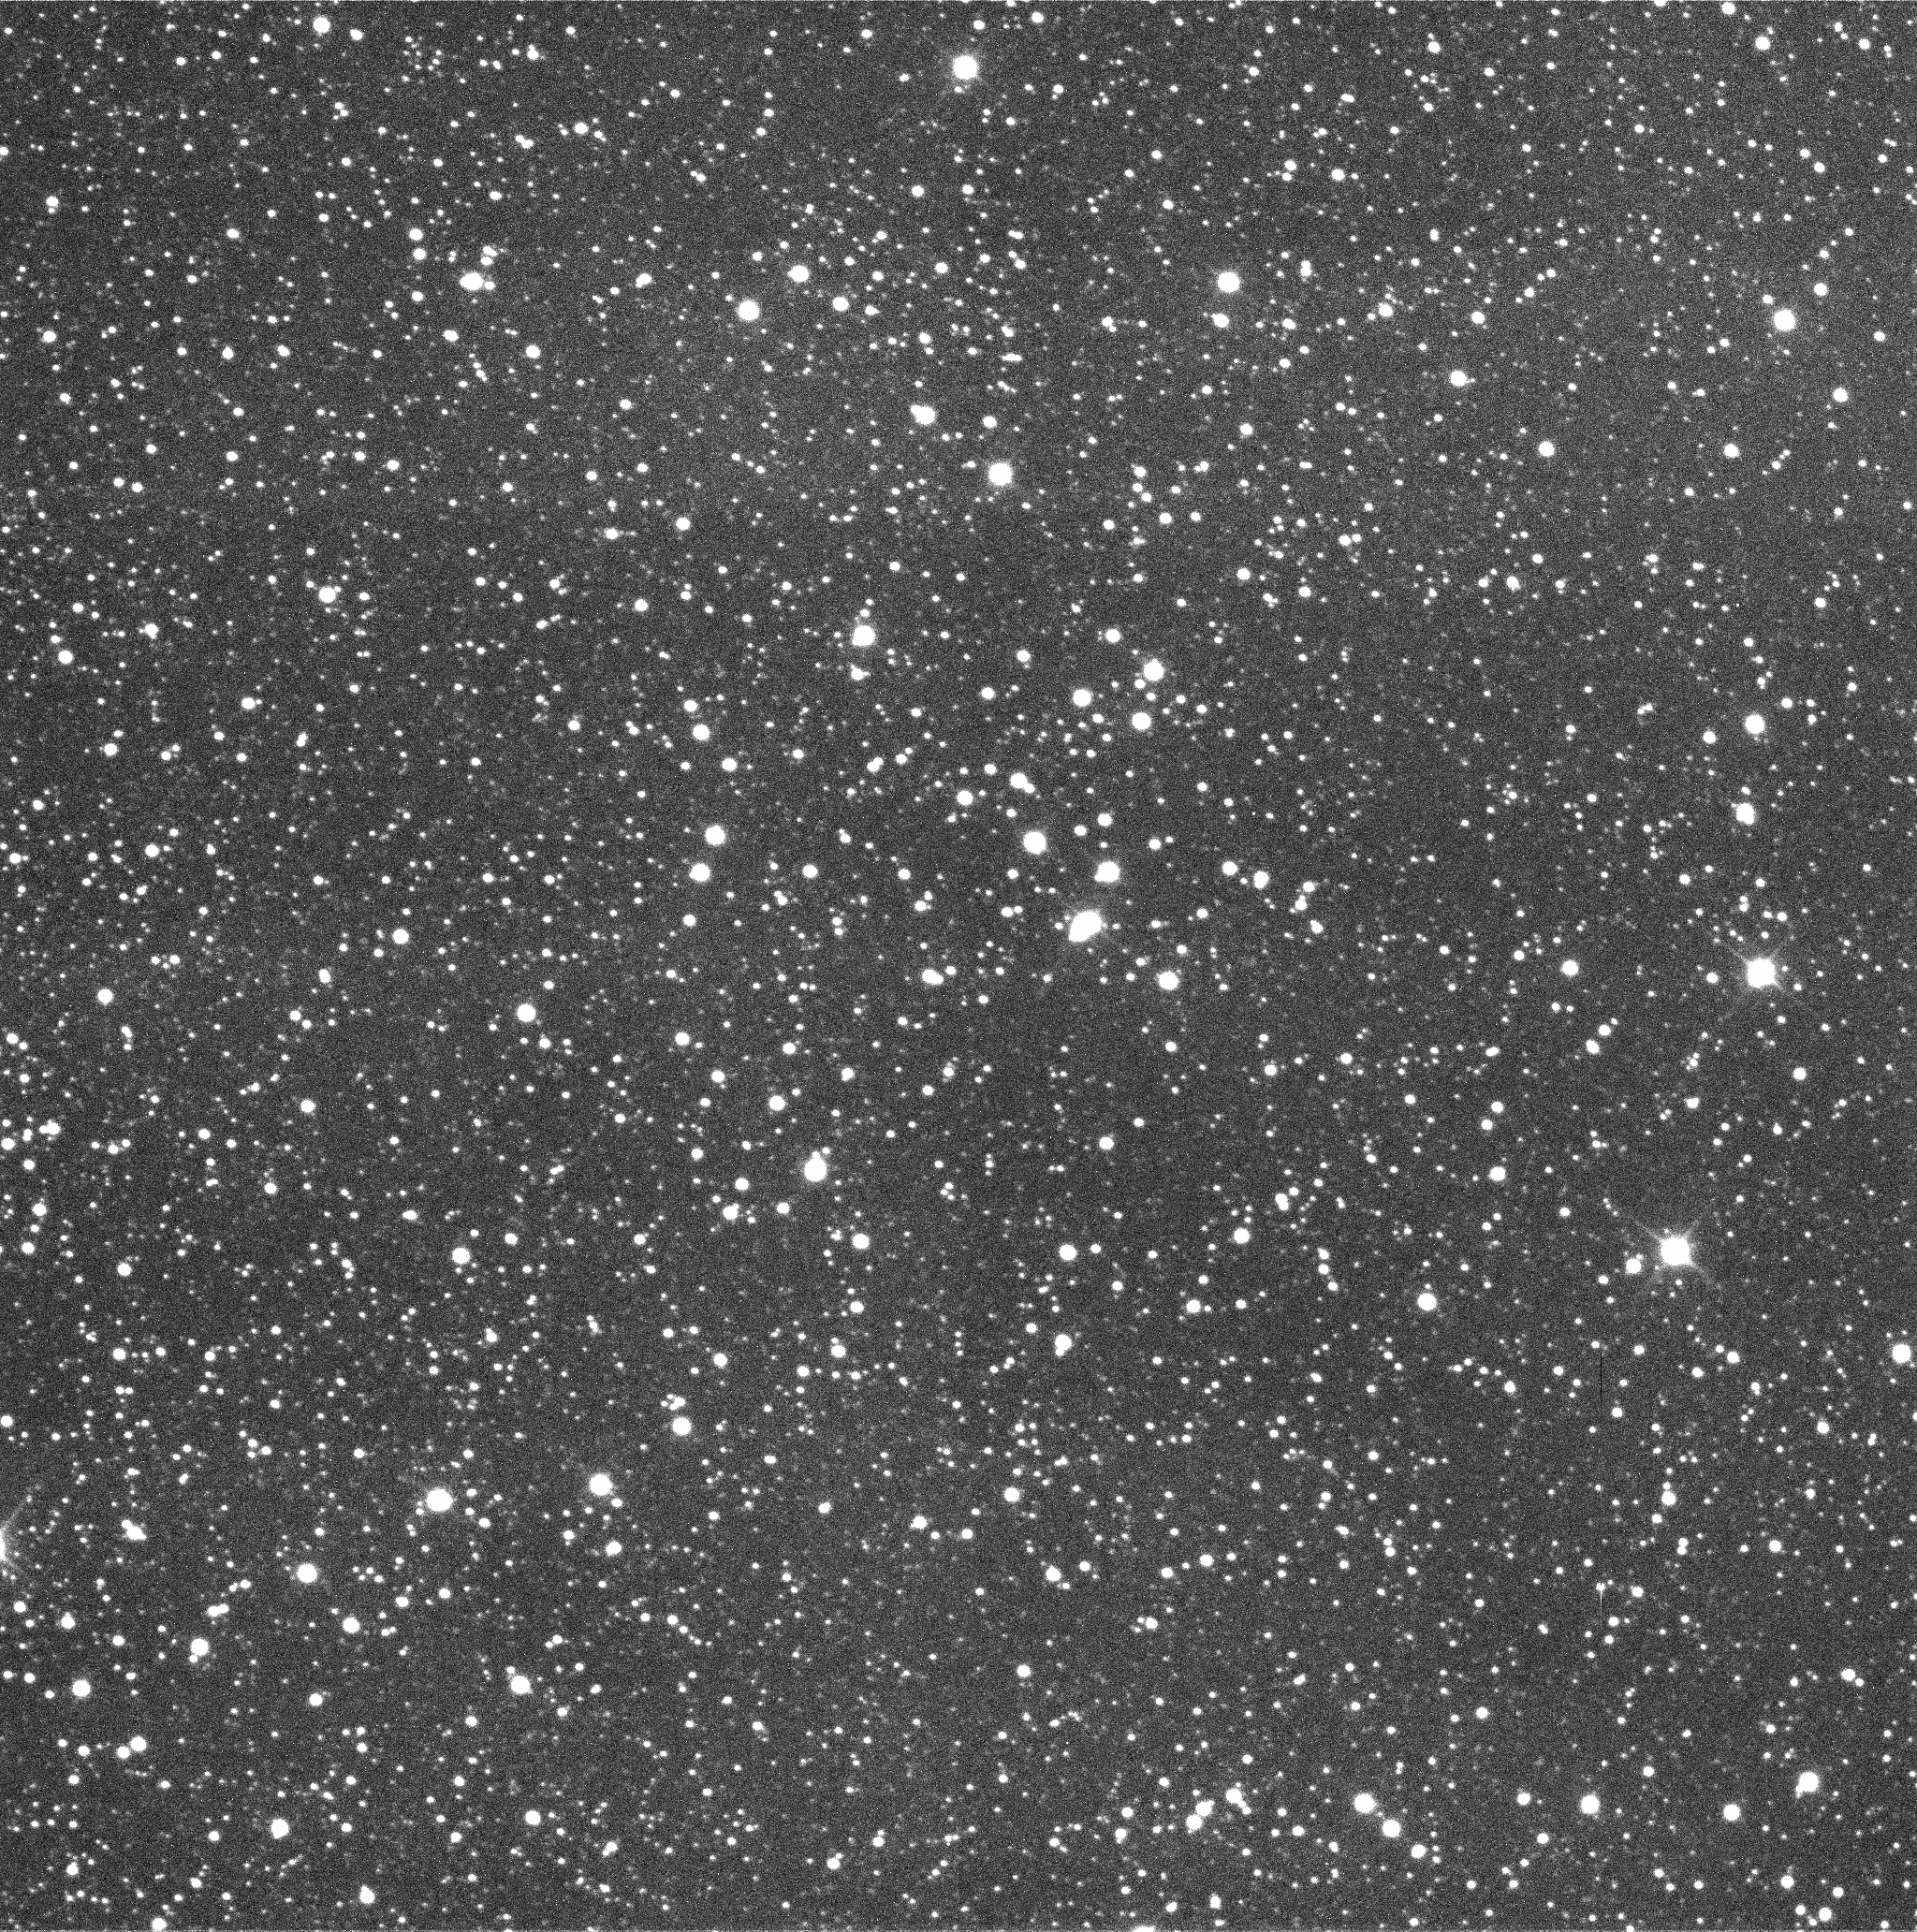
\includegraphics[width=.4\linewidth]{Images/Raw_rSDSS.png}}\quad
      \subfloat[][gSDSS]{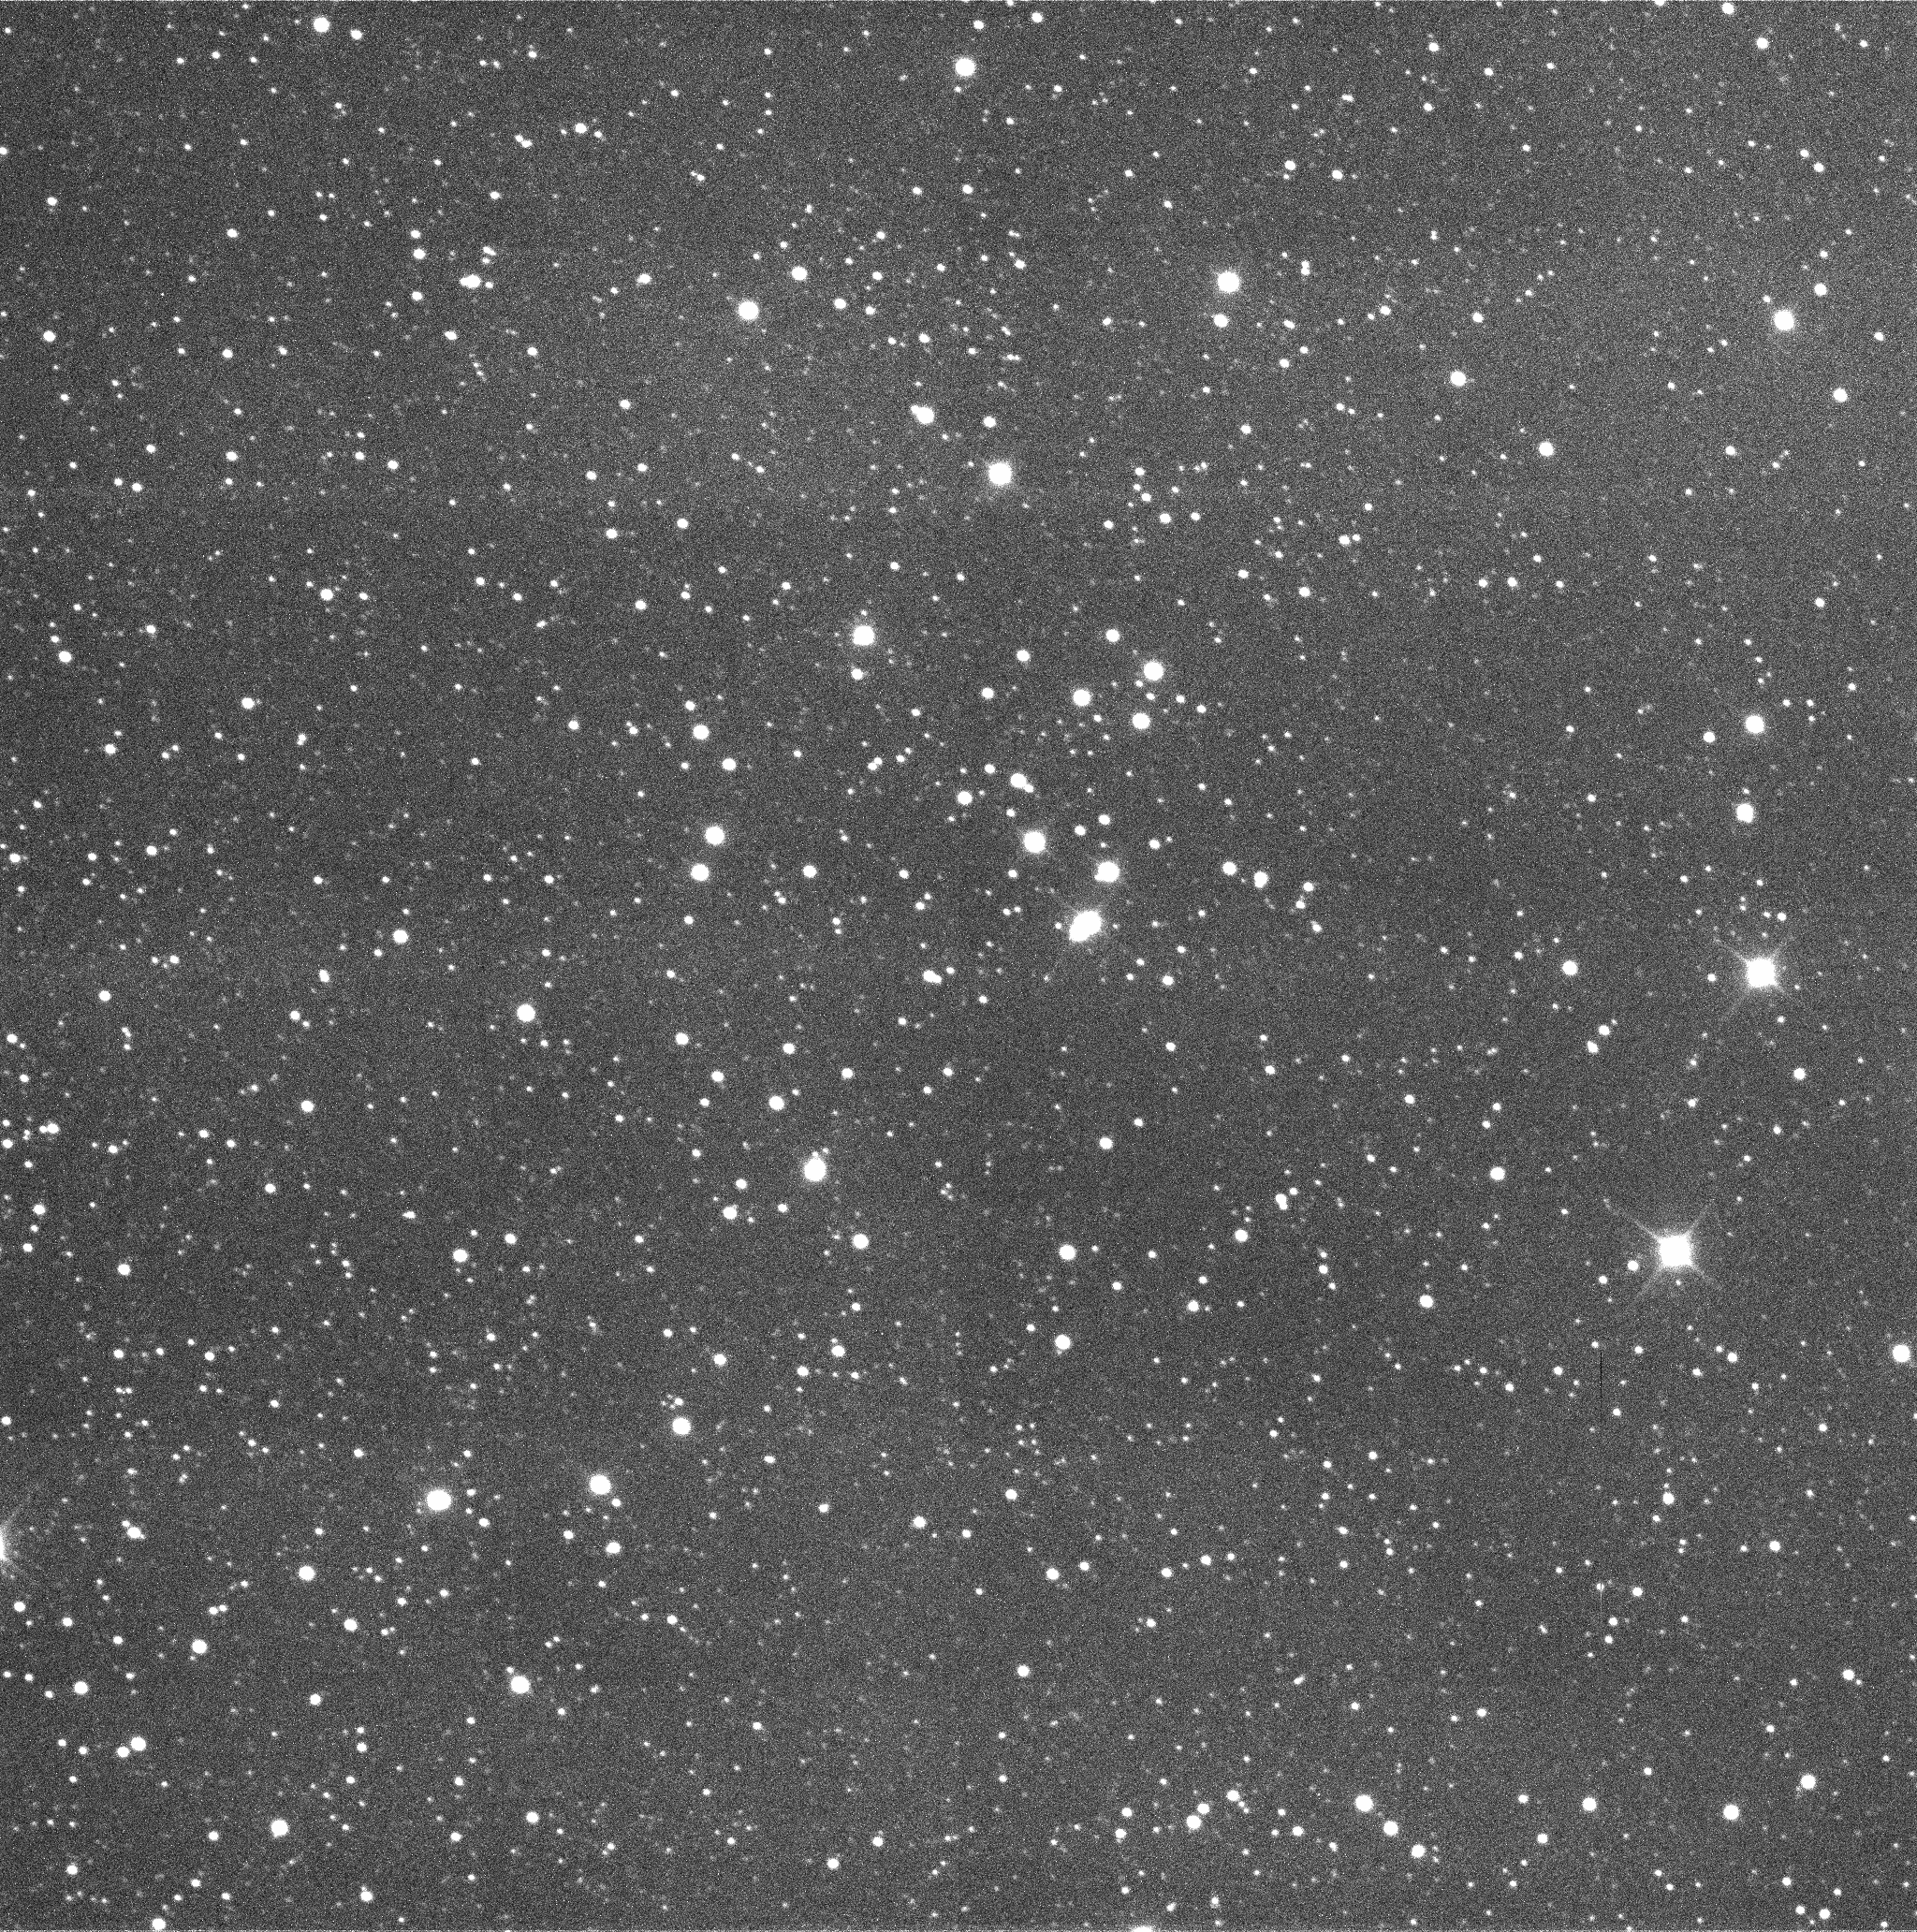
\includegraphics[width=.4\linewidth]{Images/Raw_gSDSS.png}}\\
      \subfloat[][Ha]{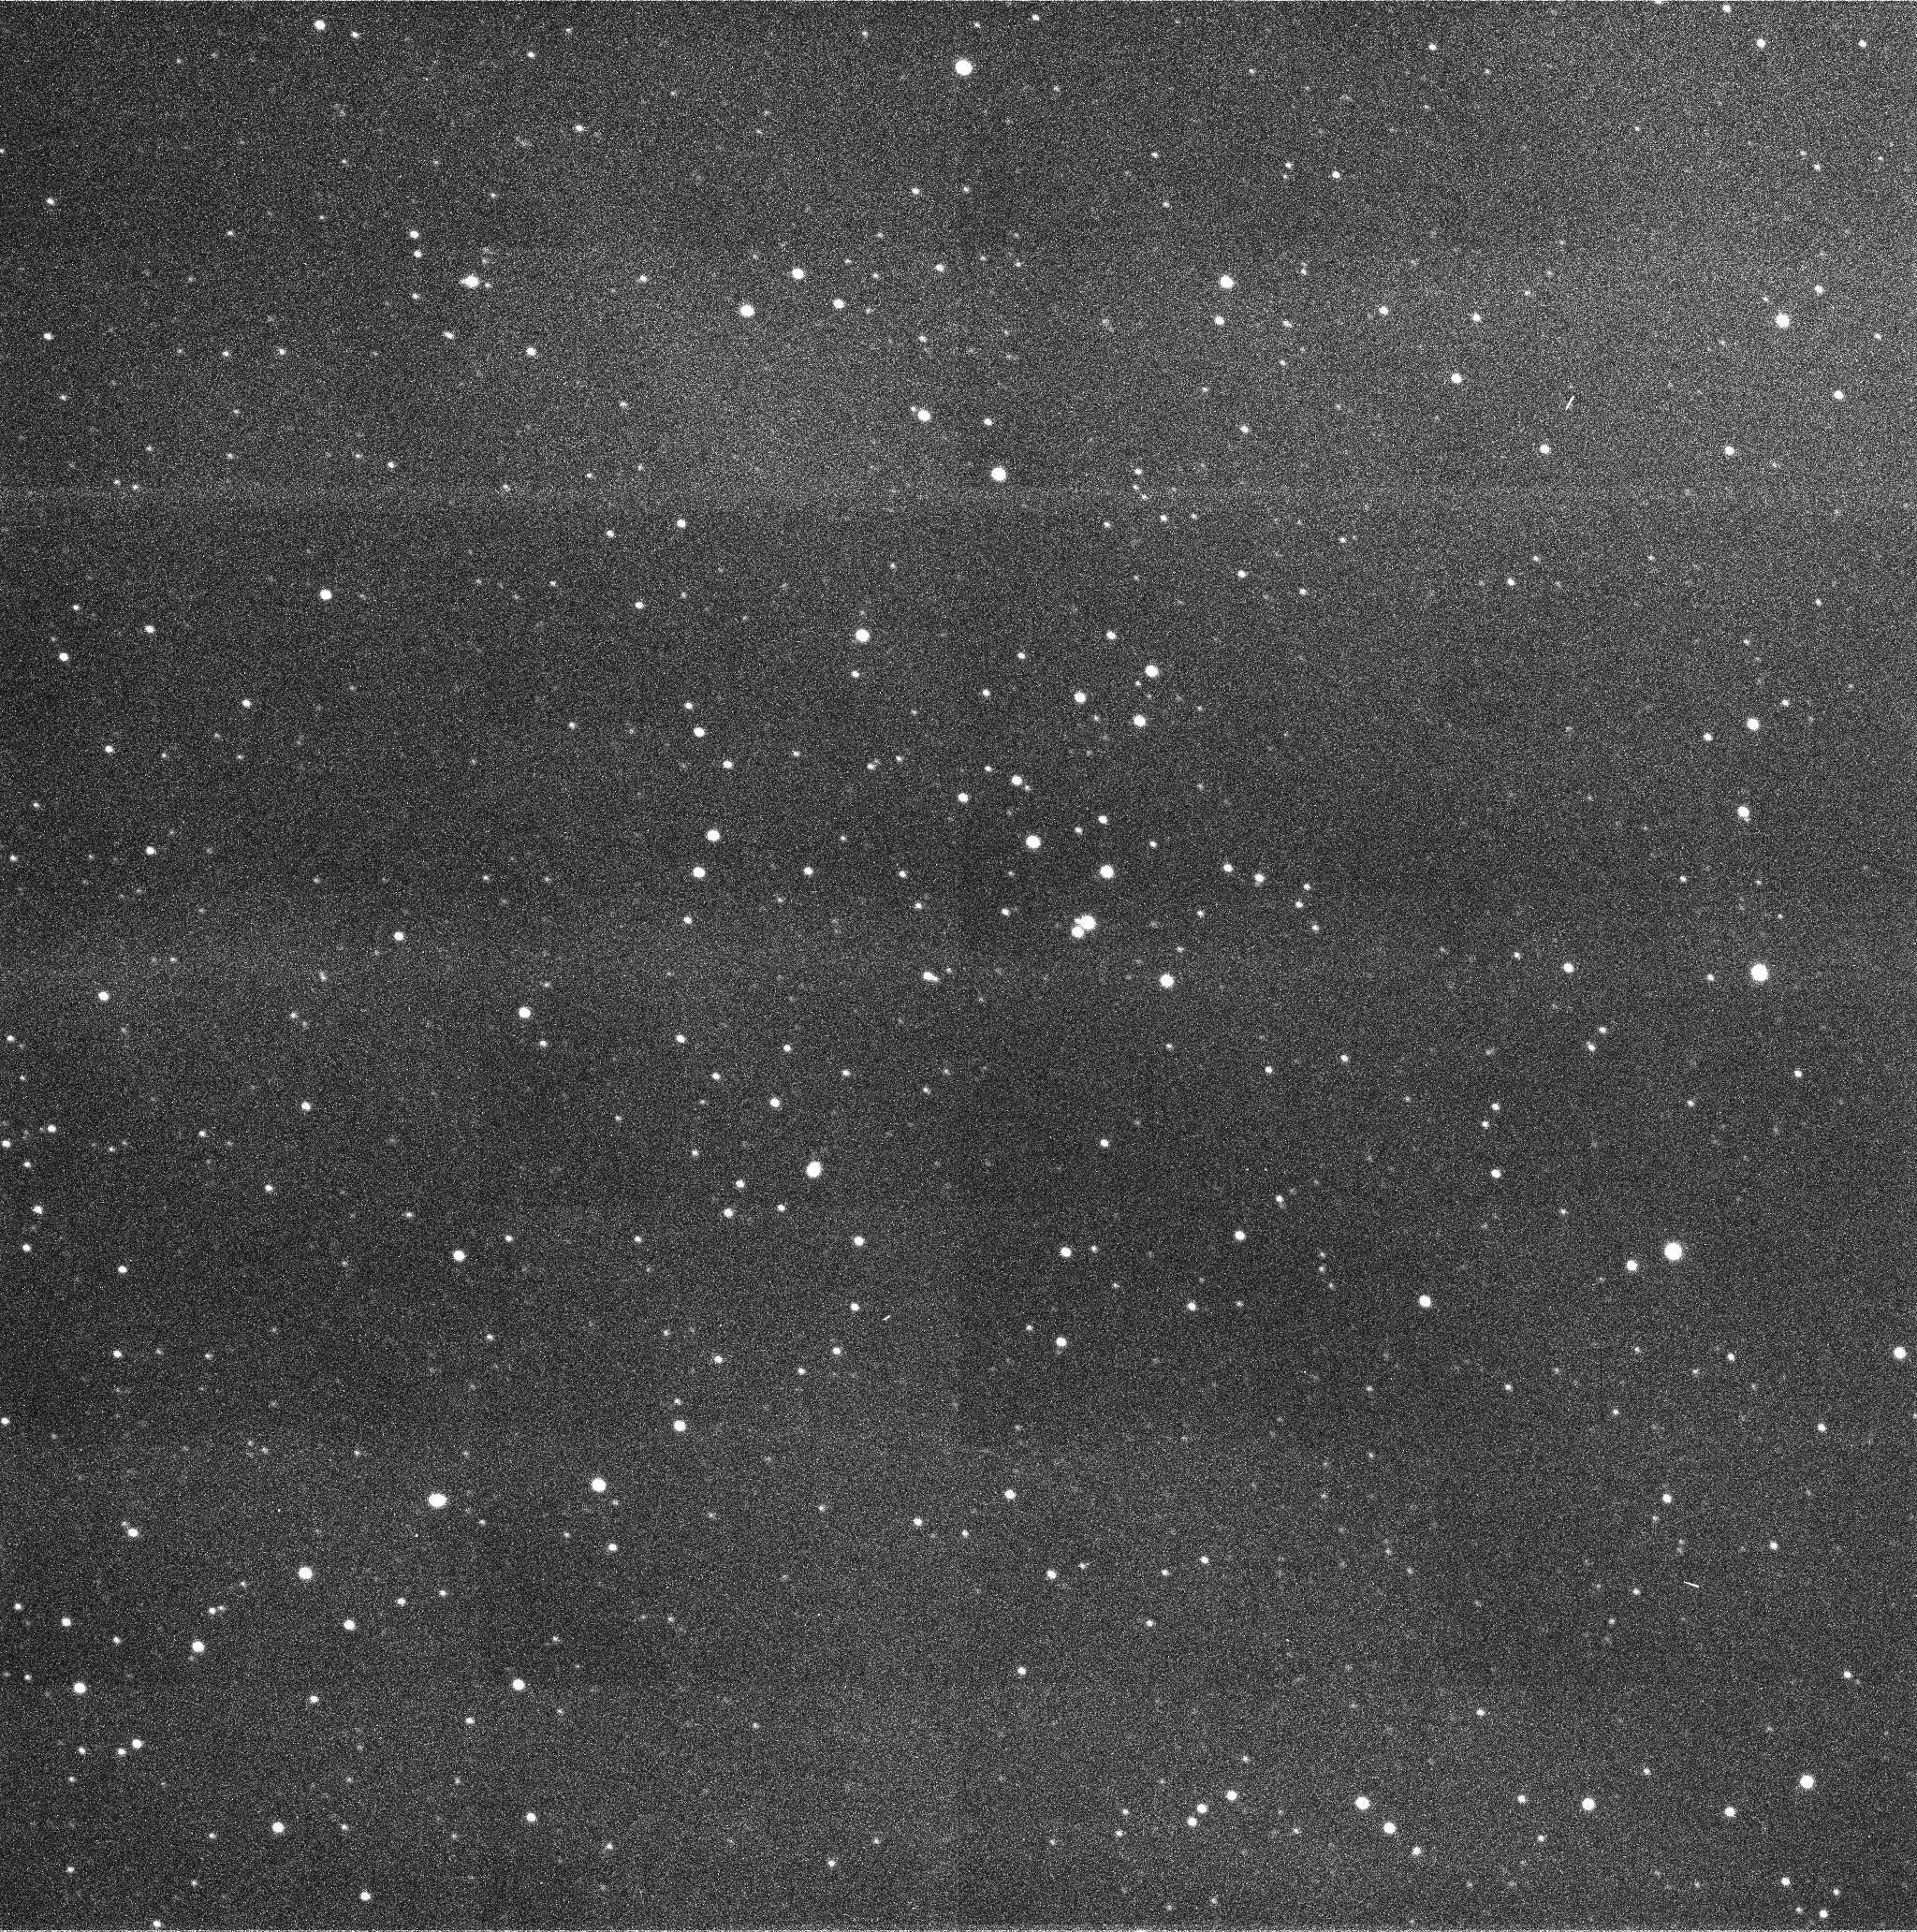
\includegraphics[width=.4\linewidth]{Images/Raw_Ha.png}}\quad
      \subfloat[][OIII]{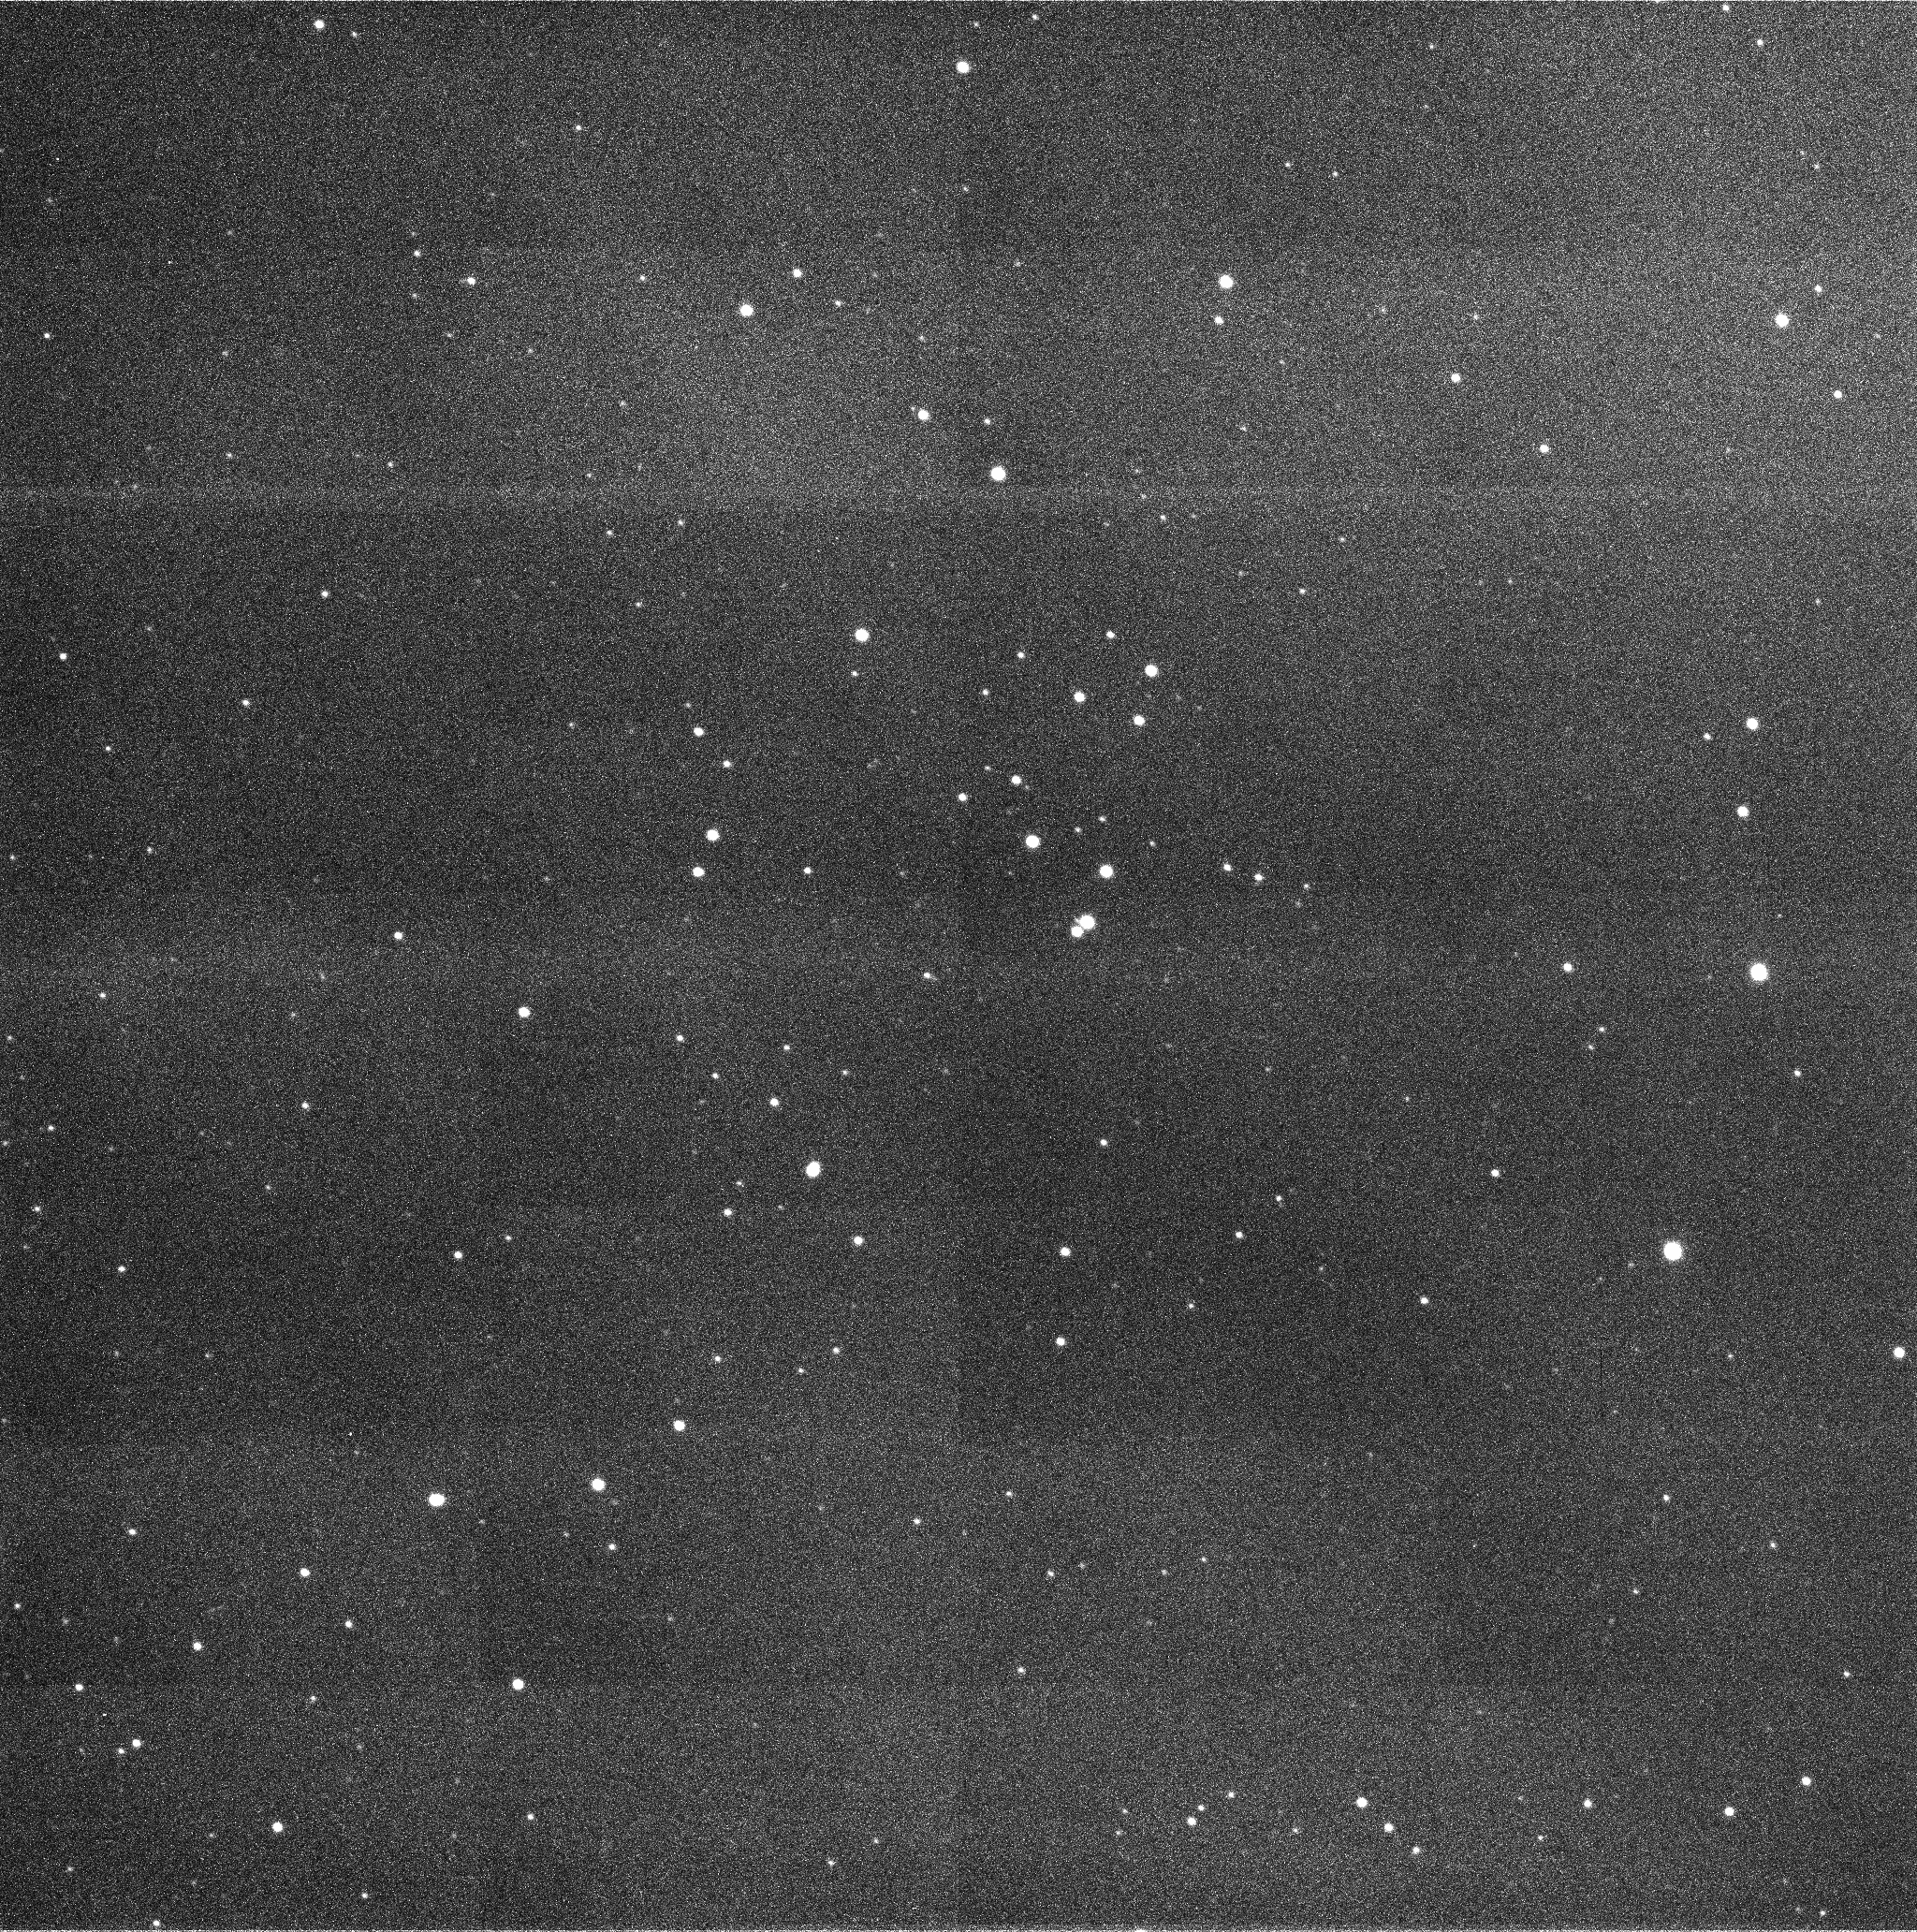
\includegraphics[width=.4\linewidth]{Images/Raw_OIII.png}}
      \caption{Raw photometric images for each filter.}
      \label{fig: Raw  Images}
    \end{figure}
    Different images were taken with different exposure times (varying from 20s to 120s) depending on the used filter; the four chosen filters were: rSDSS, gSDSS, Ha and OIII. A sample of the raw images taken on site can be seen at figure \ref{fig: Raw  Images}.
    %%%%%%%%%%%%%%%%%%%%%%%%%%%%%%%%%%%%%%%%%%%%%%%%%%%%%%%%%%%%%%%%%%%%%%%%%%%%%%%%%%%%%%%%%
    \section{Image reduction and calibration}\label{sec: Image reduction and calibration}
    It can be seen from the images in figure \ref{fig: Raw  Images} that there is great room for improvement, for starters, each of them (with varying degrees of notoriety) has a very obvious structure not originating from the sky. In order to clean this images, a reduction process was made to them.  As stated in the \textit{CCD Data Reduction Guide} (\cite{CCD_Guide}) the composition of a raw astronomical image can be interpreted as
    \begin{equation}
        \text{raw image} =\text{bias}+\text{noise}+\text{dark current}+\text{flat}\,\times\left(\text{sky}+\text{stars}\right)
    \end{equation}
    and thus, in order to get cleaner images (that is, a image consisting of sky, stars and random noise) a process to remove the bias, dark current and flat fielding must take place.
    
    The image reduction process was made by following the aforementioned \textit{CCD Data Reduction Guide}, which uses the \textit{ccdproc} python library (\cite{Python}). The complete python script alongside all the image files can be found at the \cite{GitHub} GitHub repository.
    \begin{figure}[H]
      \centering
      \subfloat[][Masterbias]{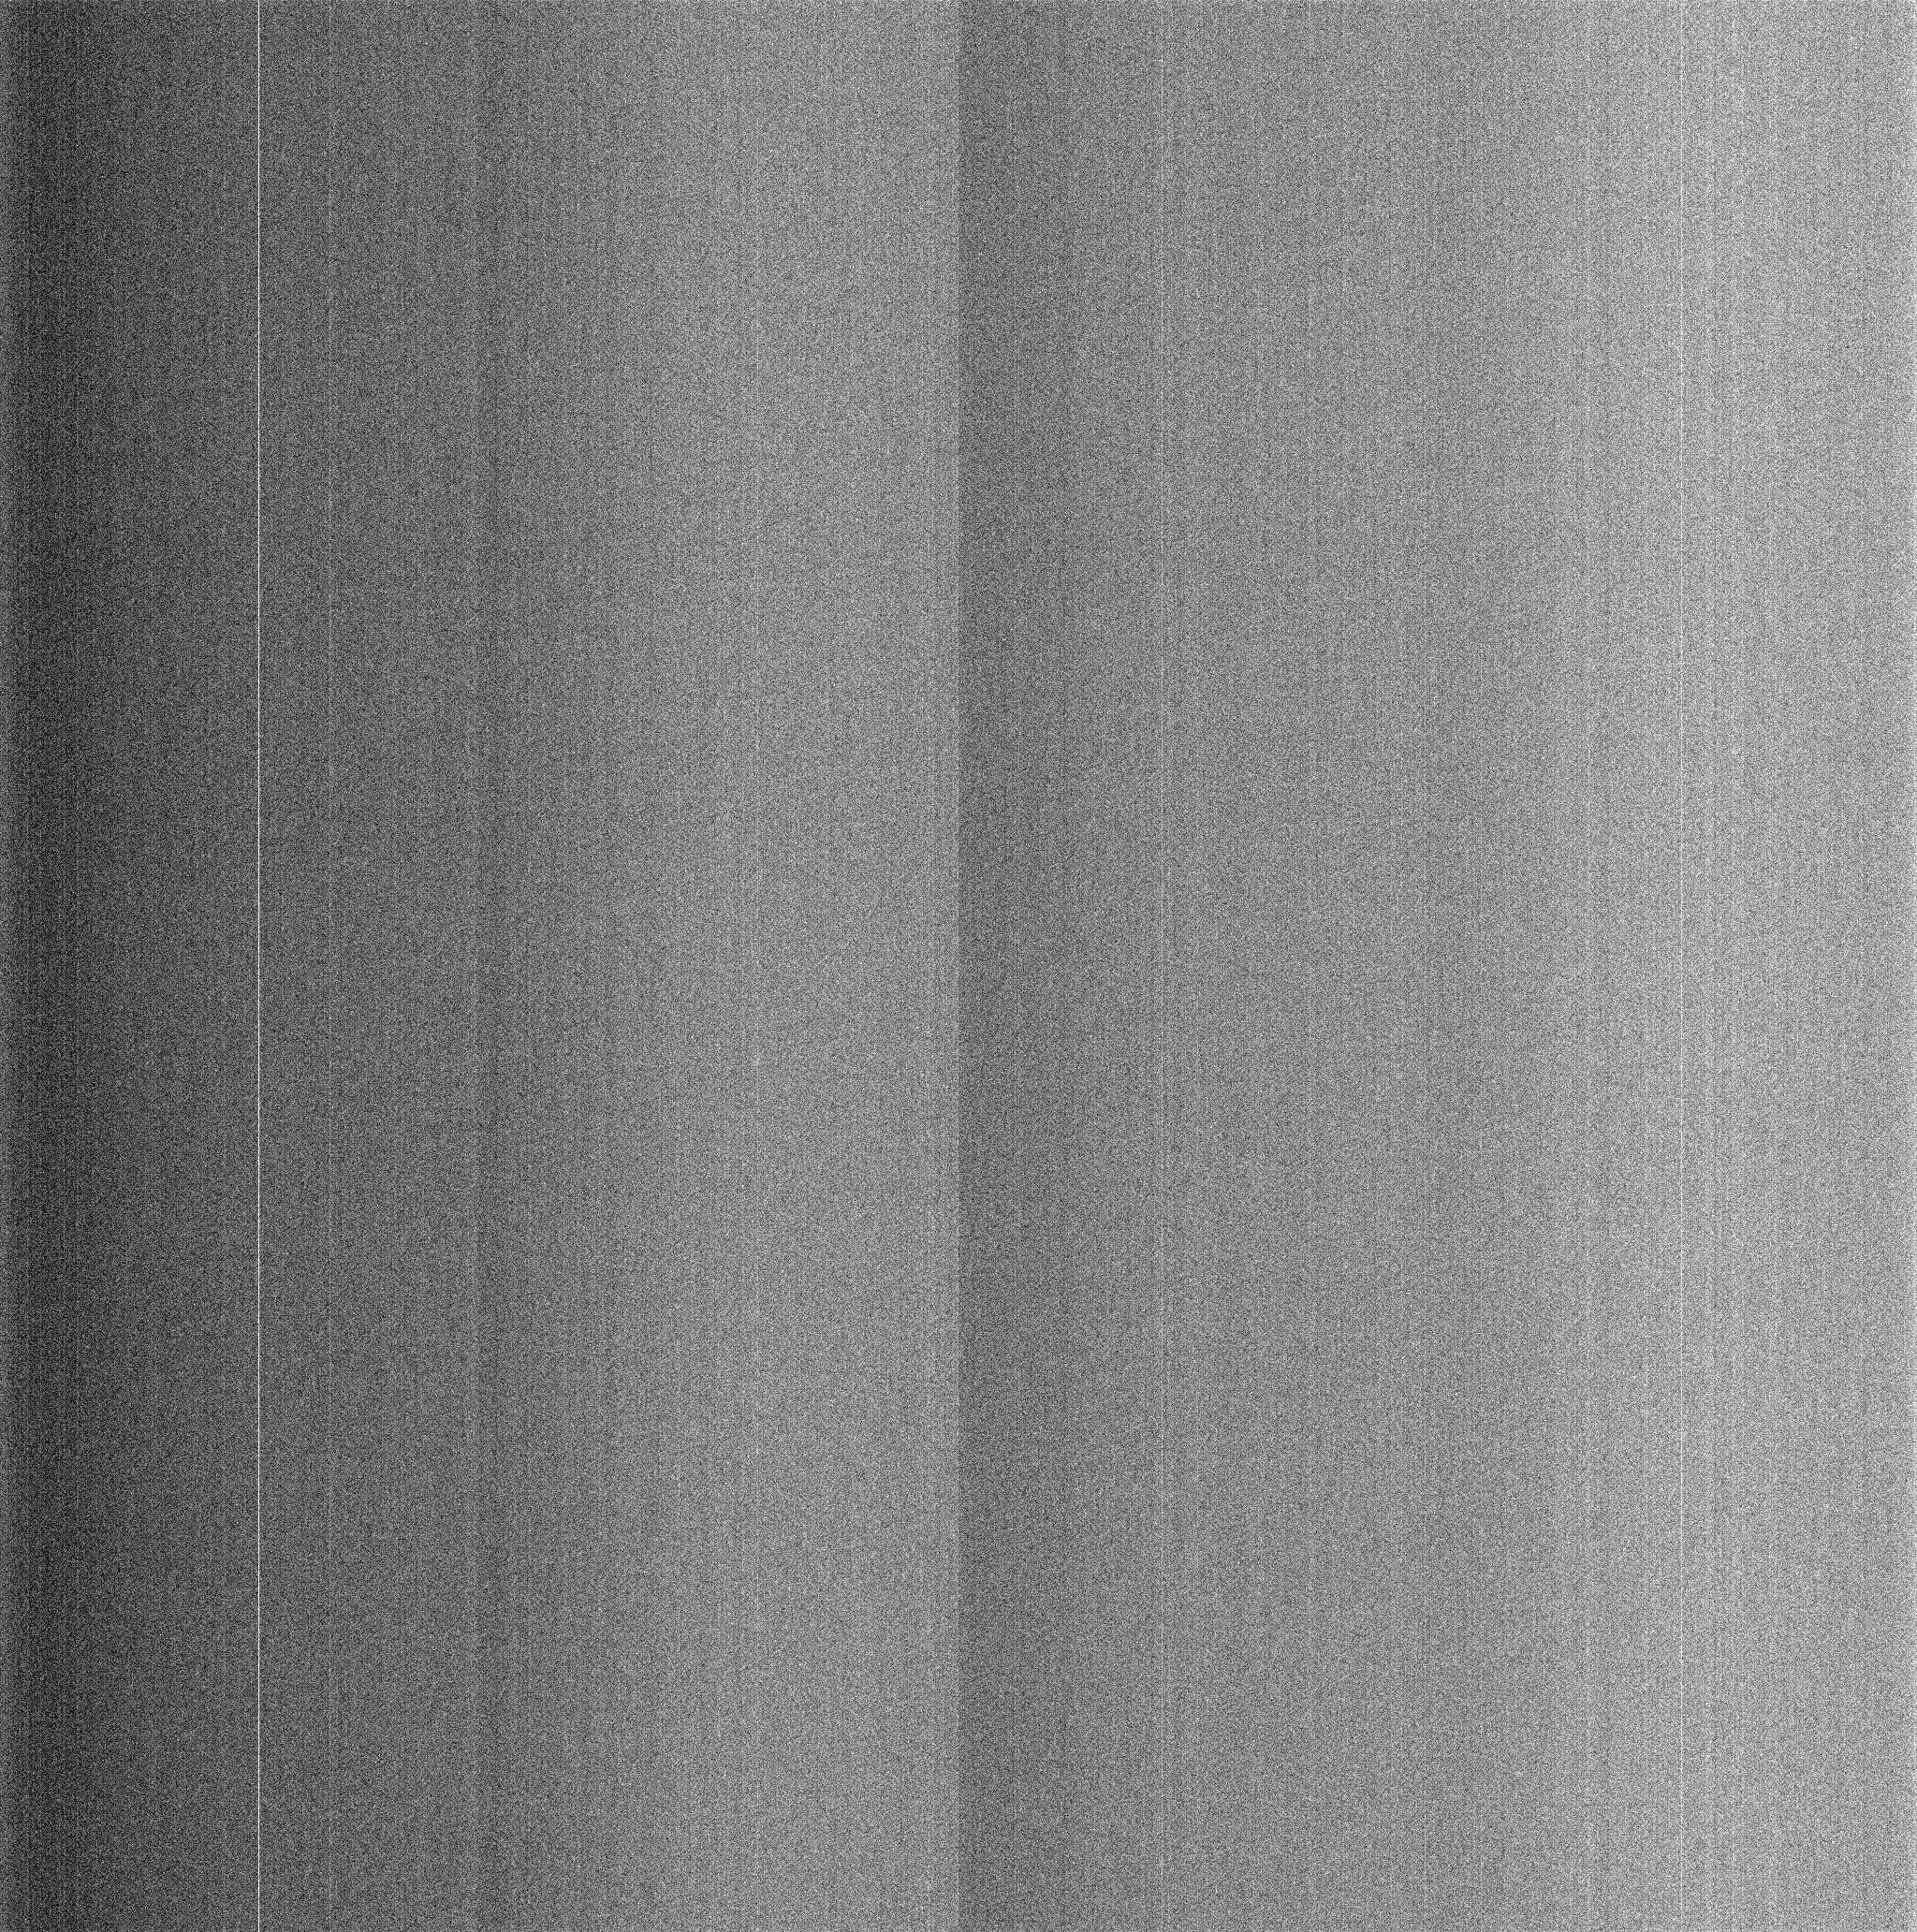
\includegraphics[width=.4\linewidth]{Images/masterbias.png}}\quad
      \subfloat[][Masterdark]{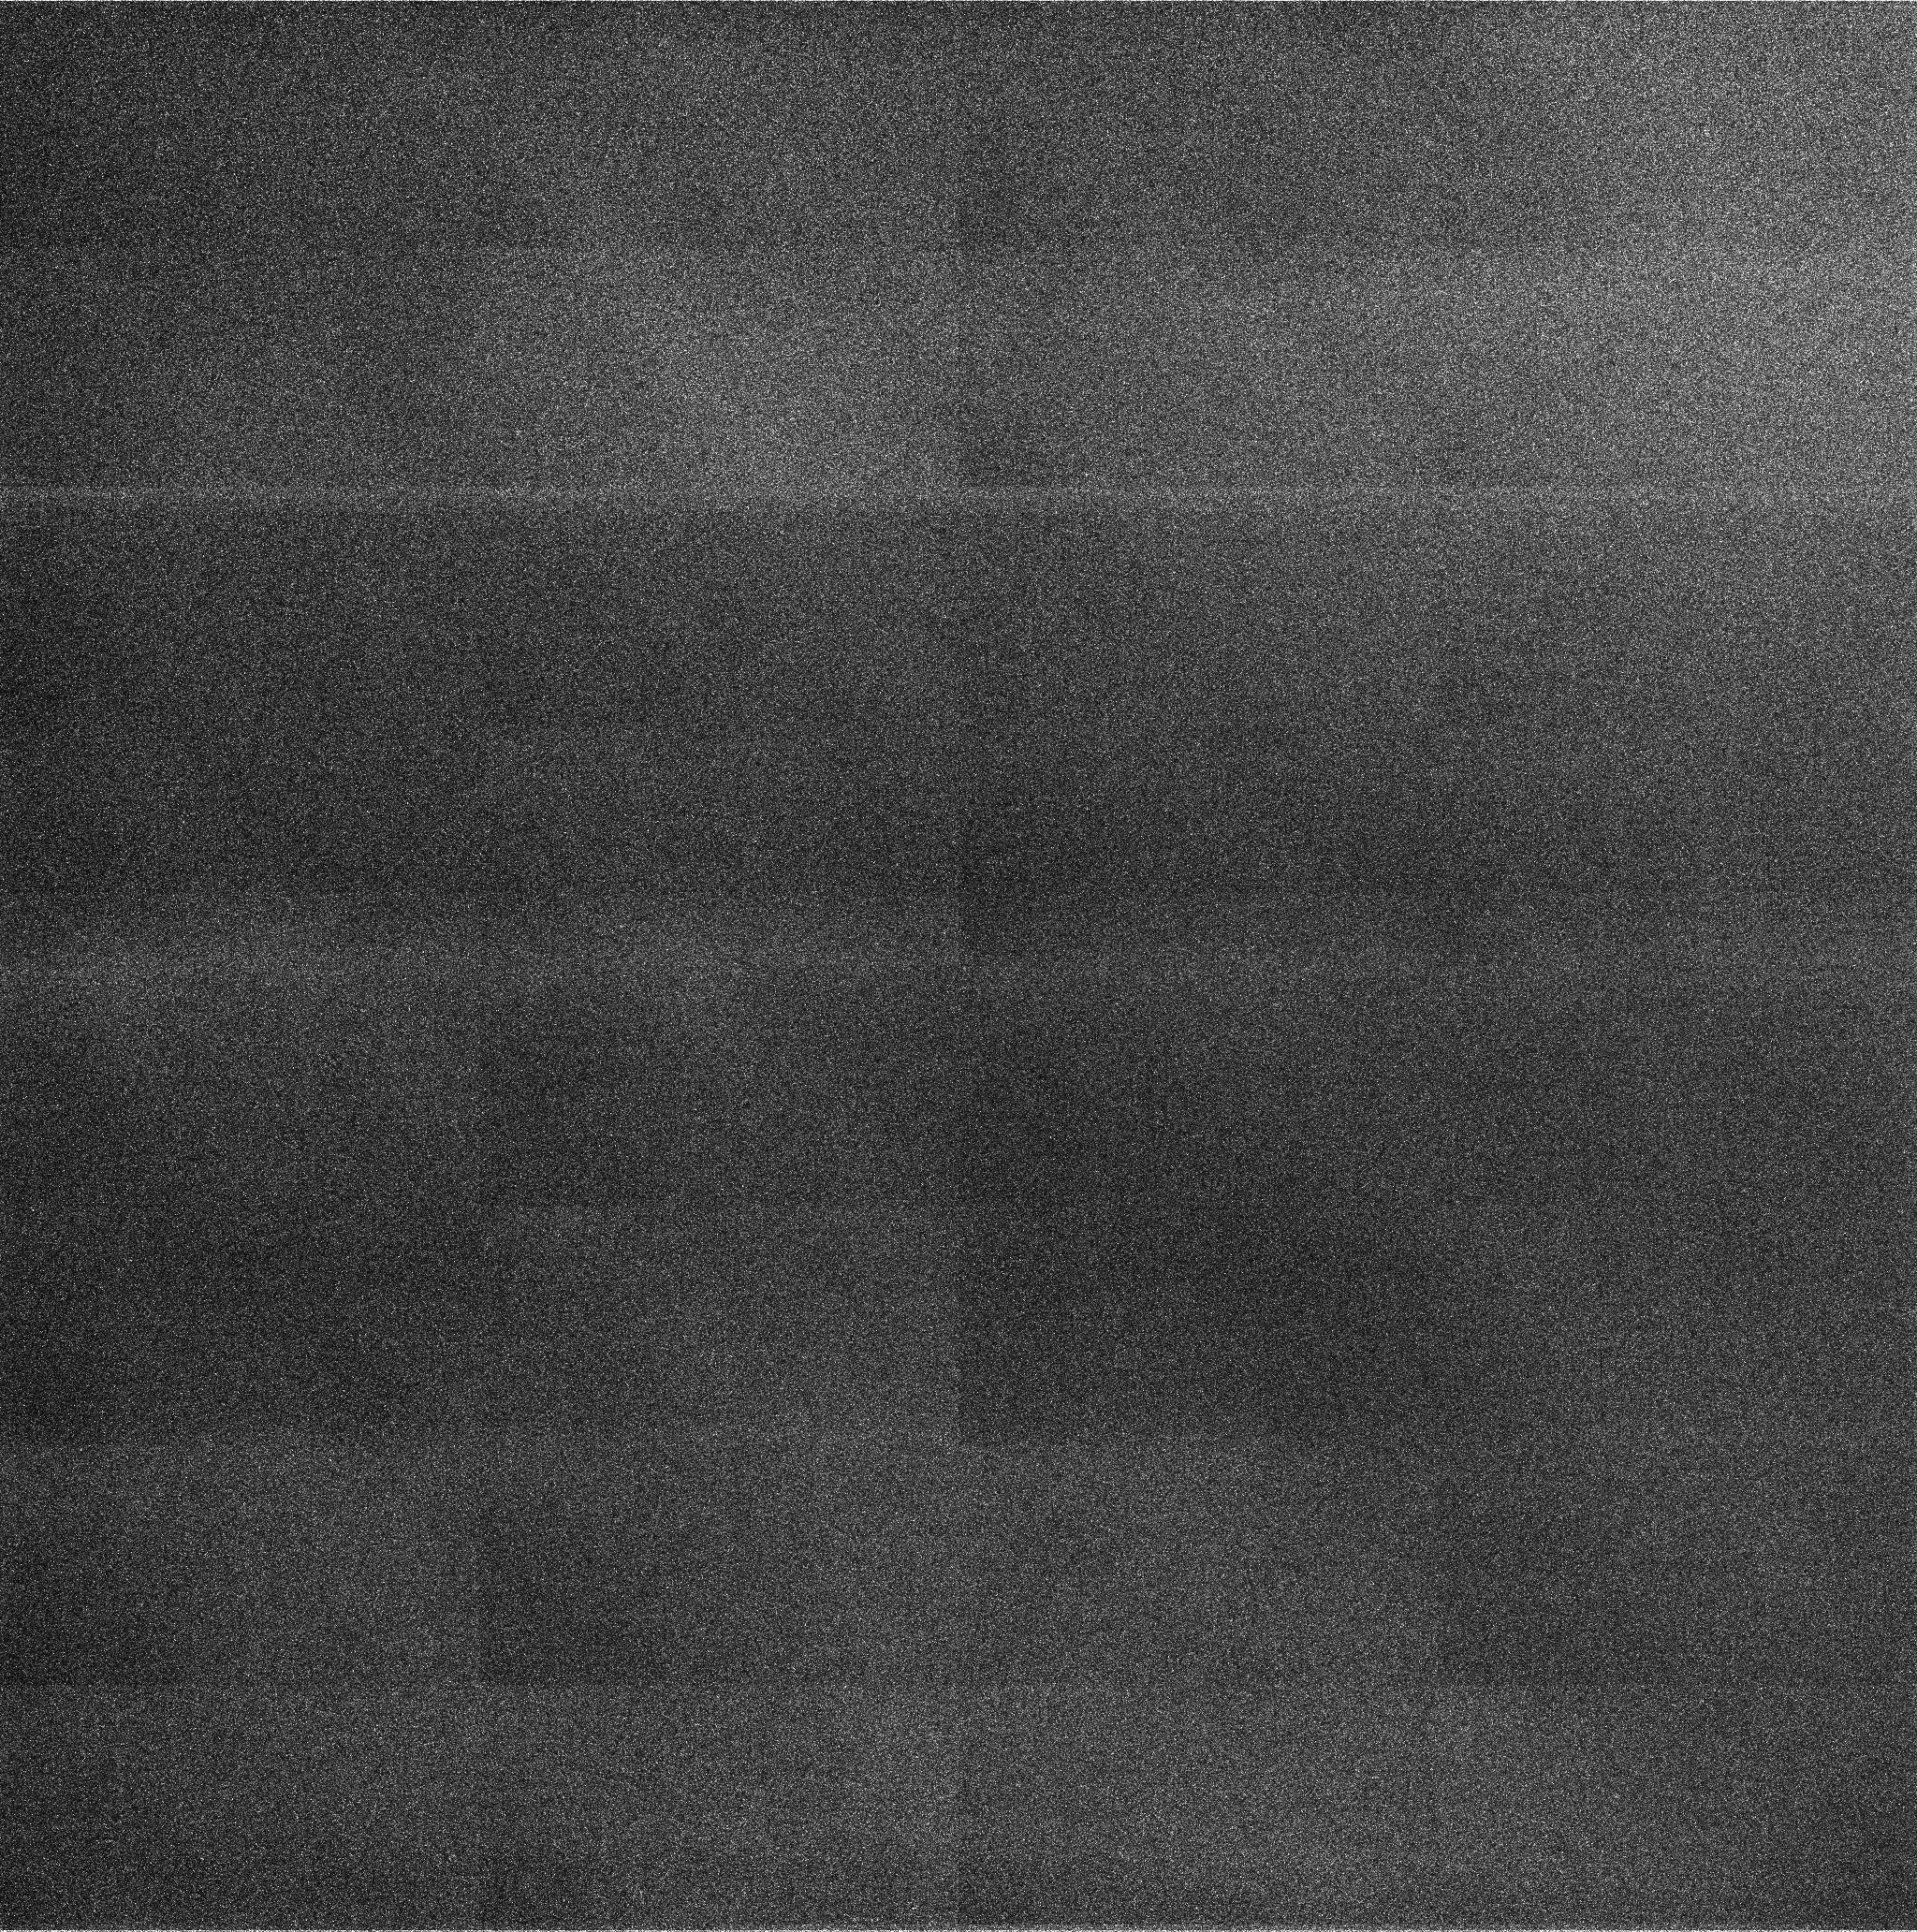
\includegraphics[width=.4\linewidth]{Images/masterdark_120s.png}}
      \caption{Images of combined bias and darks.}
      \label{fig: Bias and Dark}
    \end{figure}
    \begin{figure}[H]
      \centering
      \subfloat[][rSDSS]{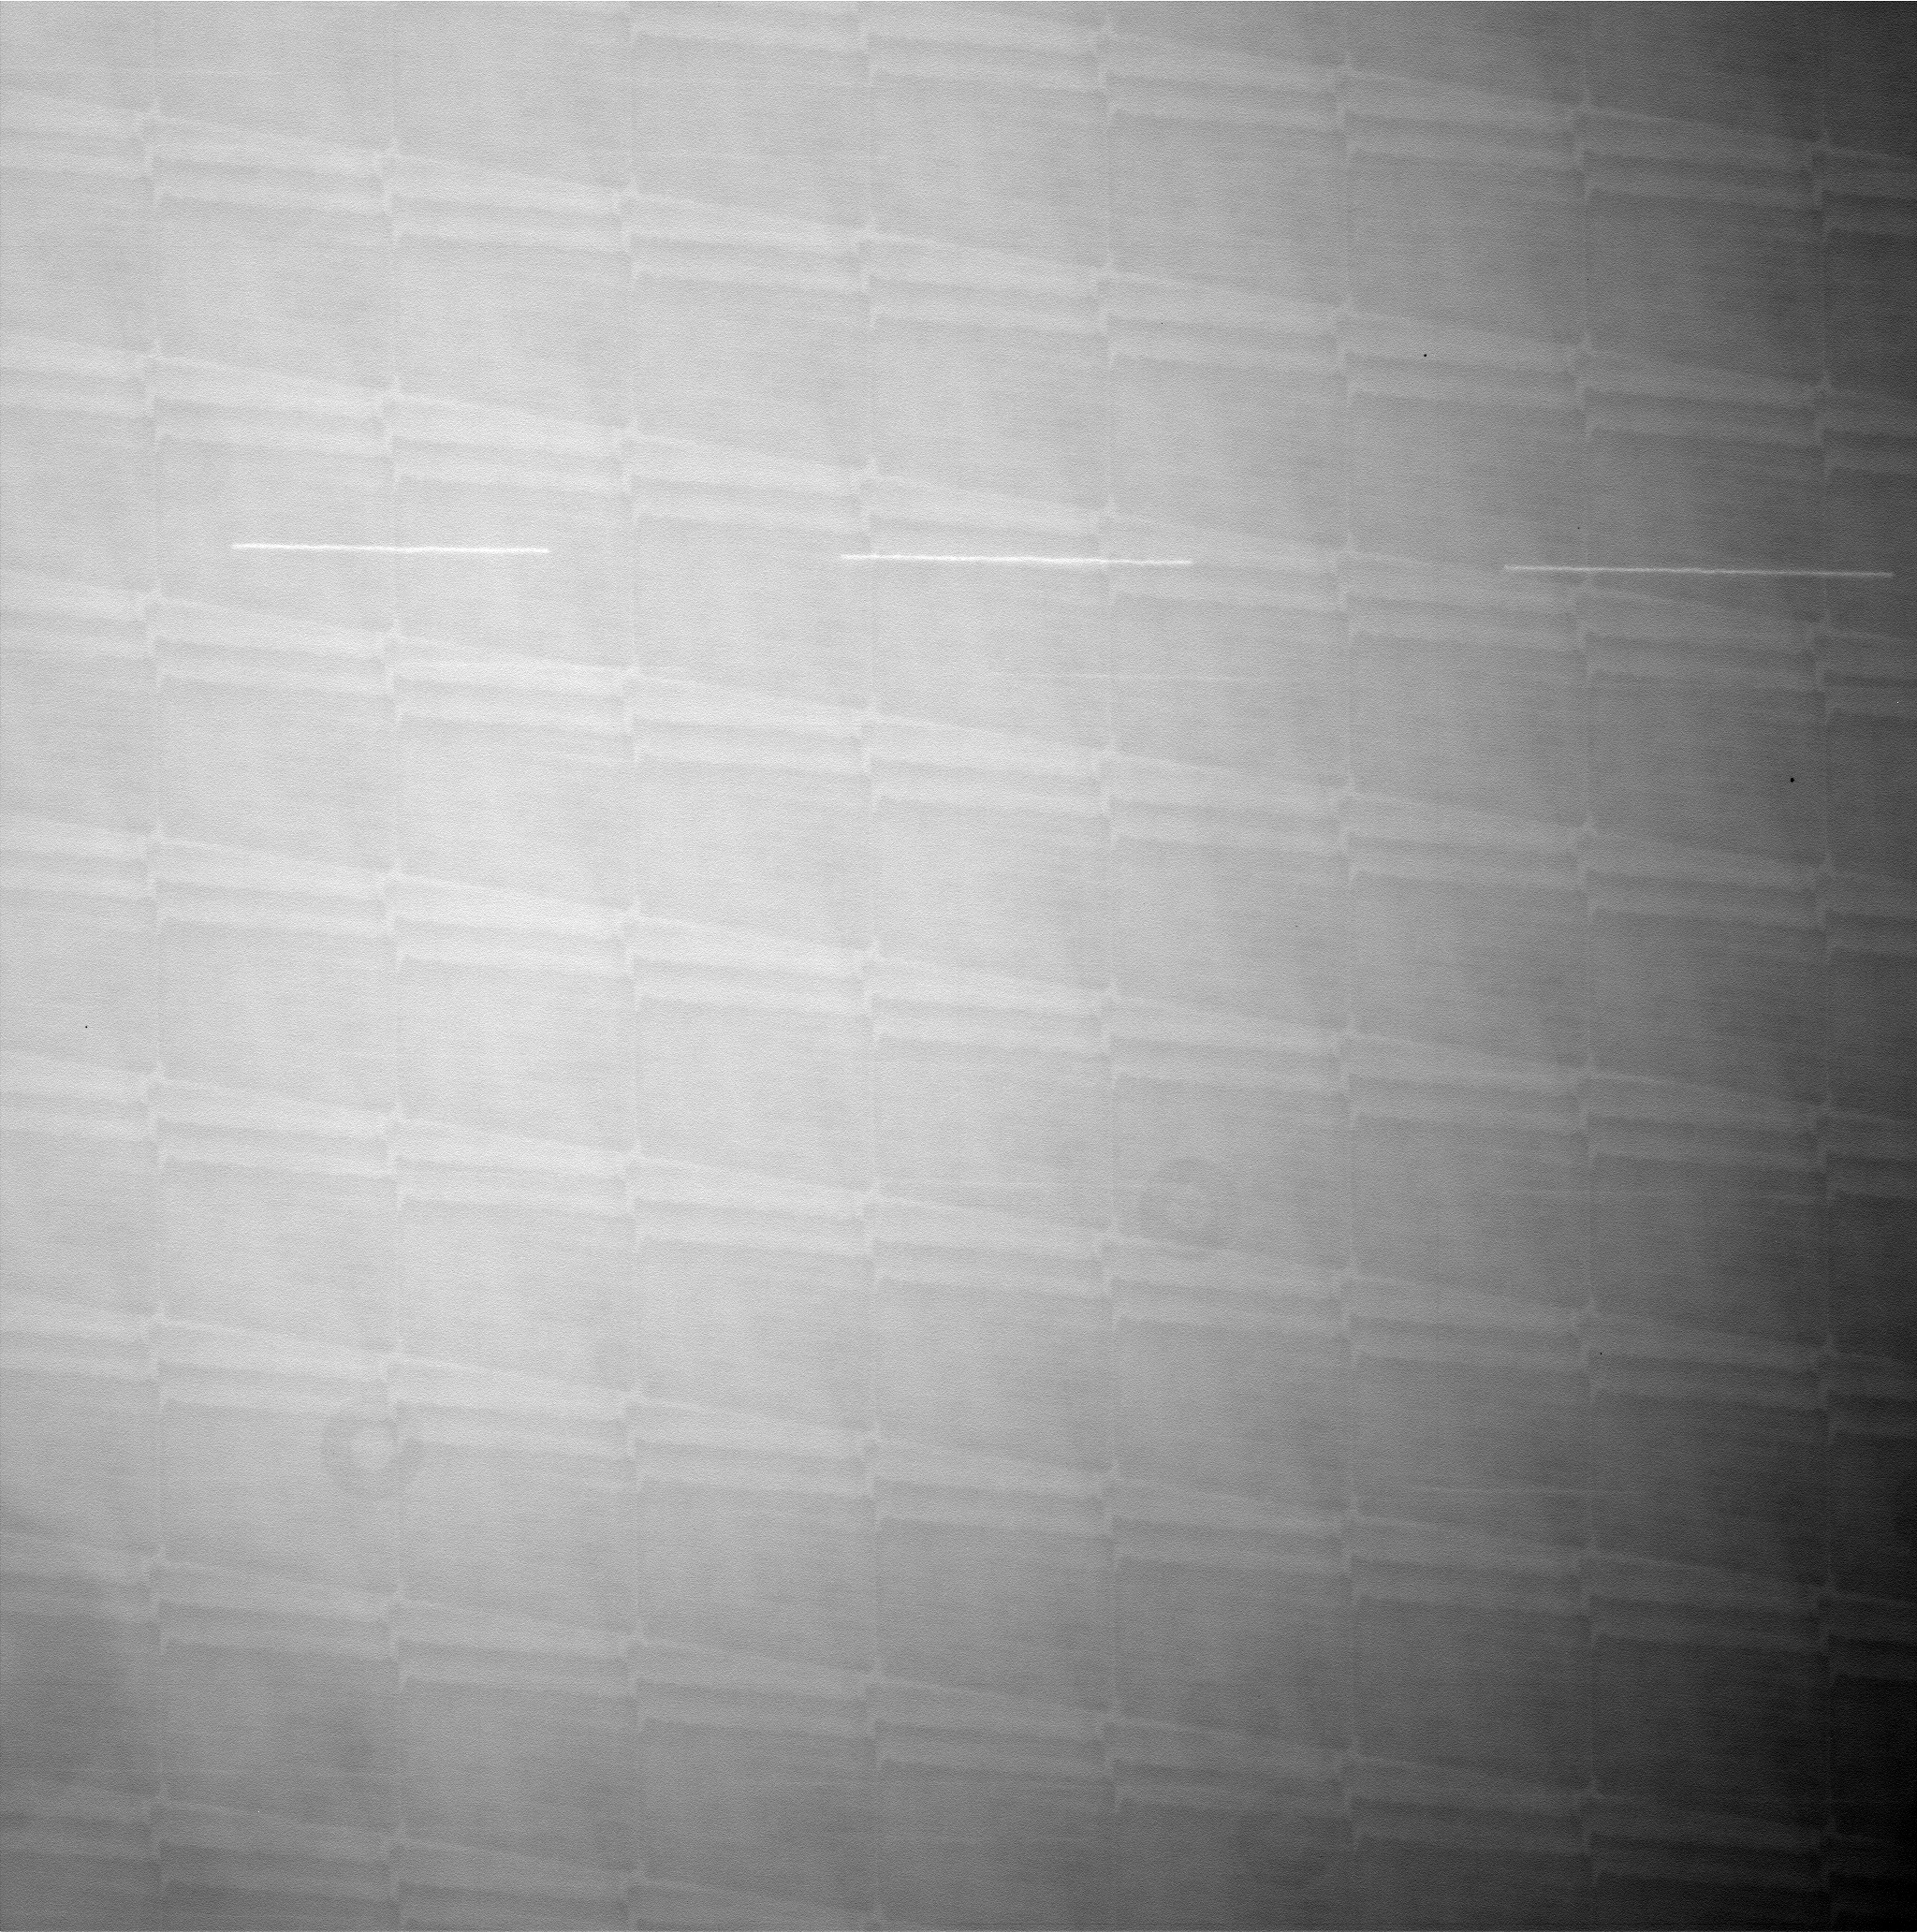
\includegraphics[width=.4\linewidth]{Images/masterflat_rSDSS.png}}\quad
      \subfloat[][gSDSS]{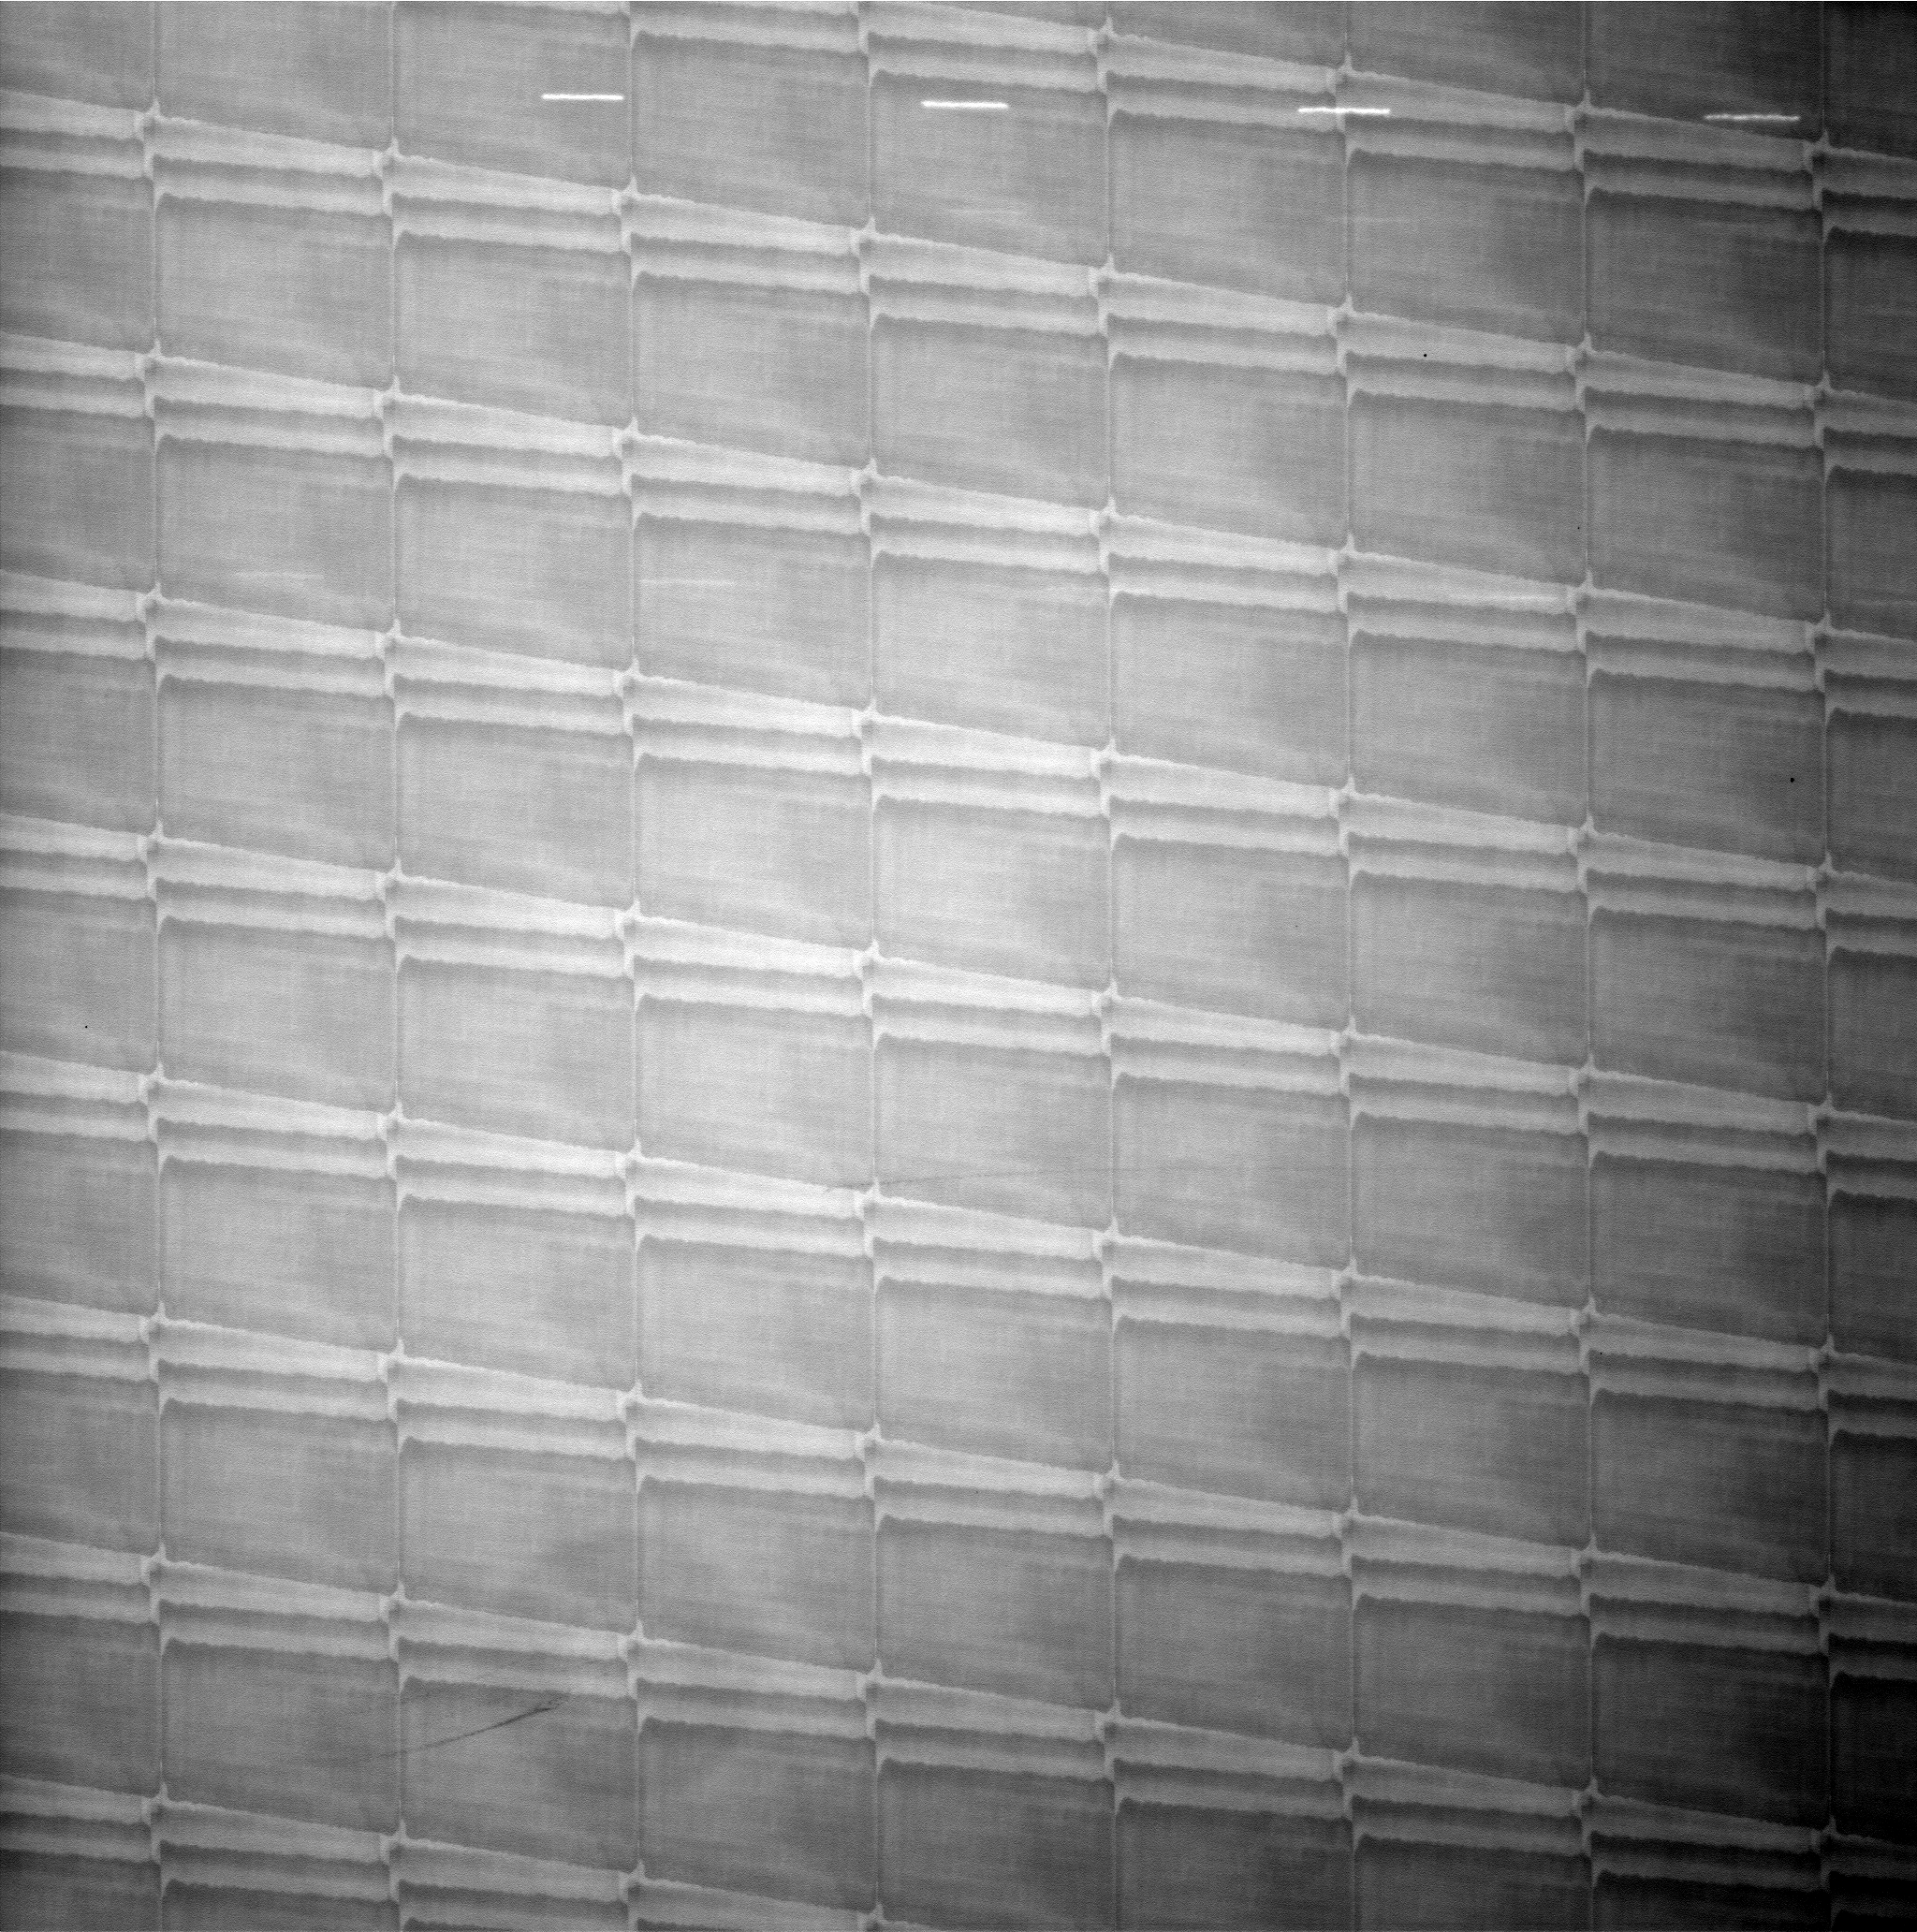
\includegraphics[width=.4\linewidth]{Images/masterflat_gSDSS.png}}\\
      \subfloat[][Ha]{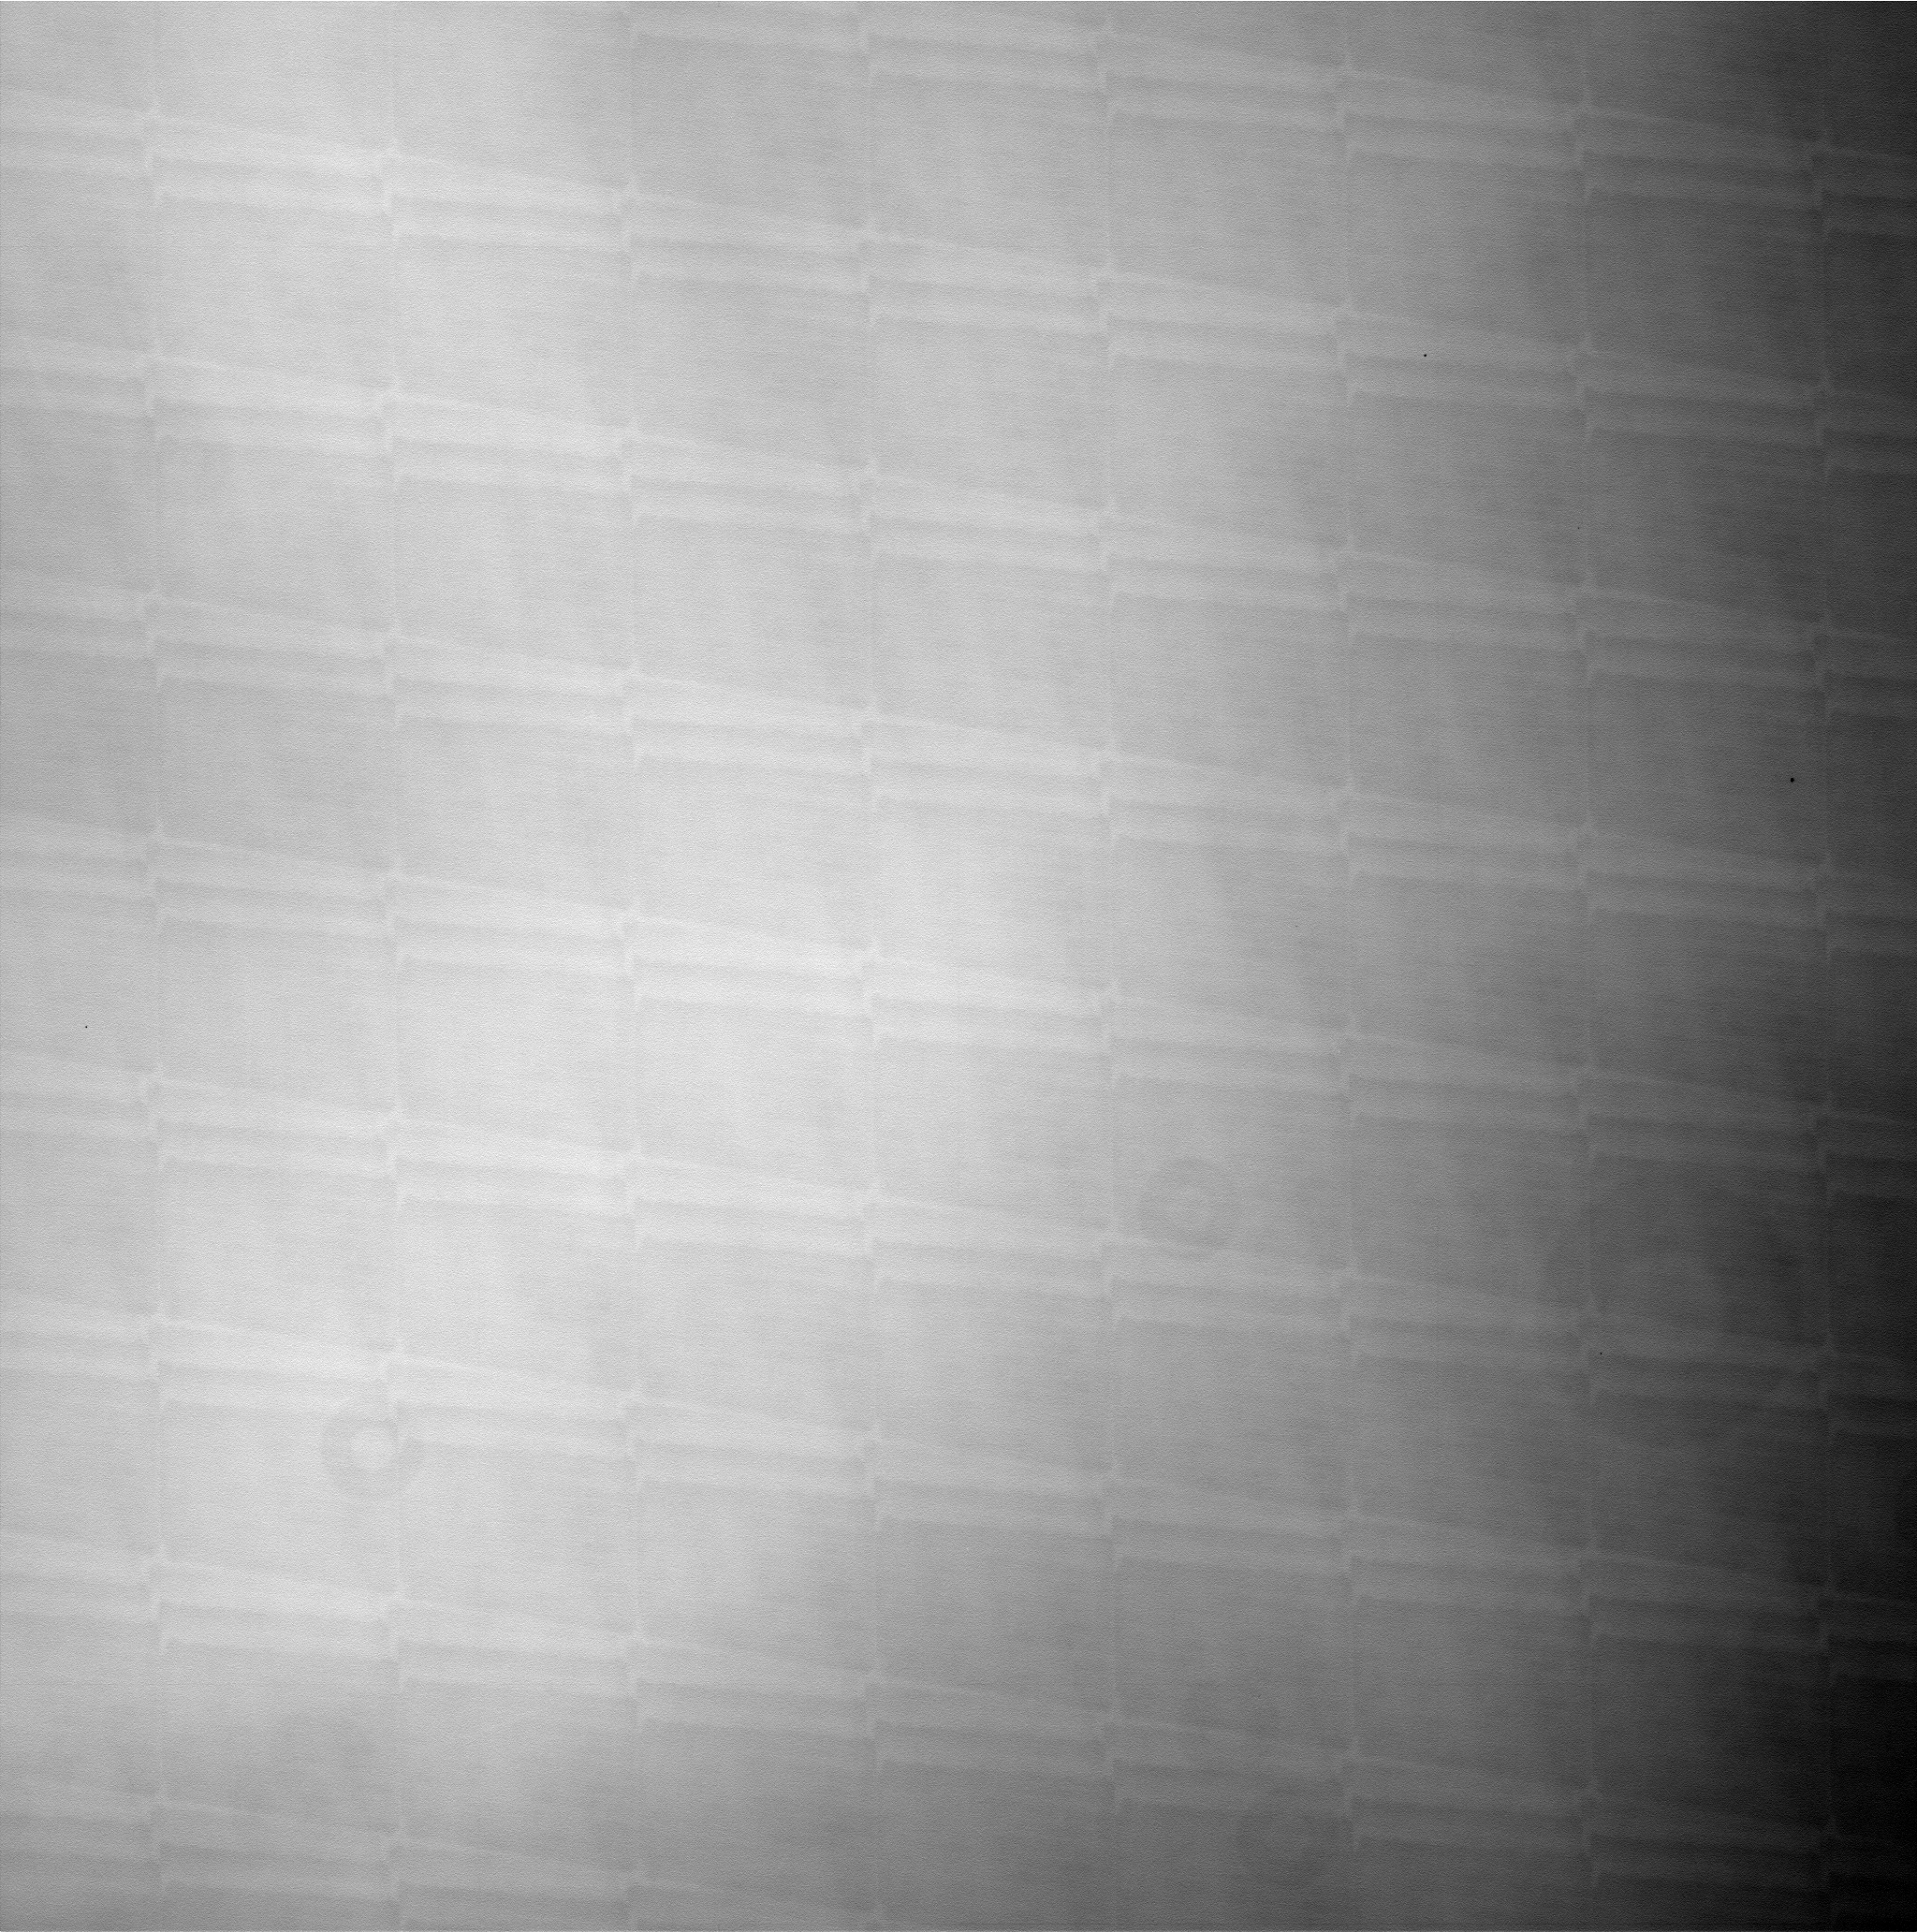
\includegraphics[width=.4\linewidth]{Images/masterflat_Ha.png}}\quad
      \subfloat[][OIII]{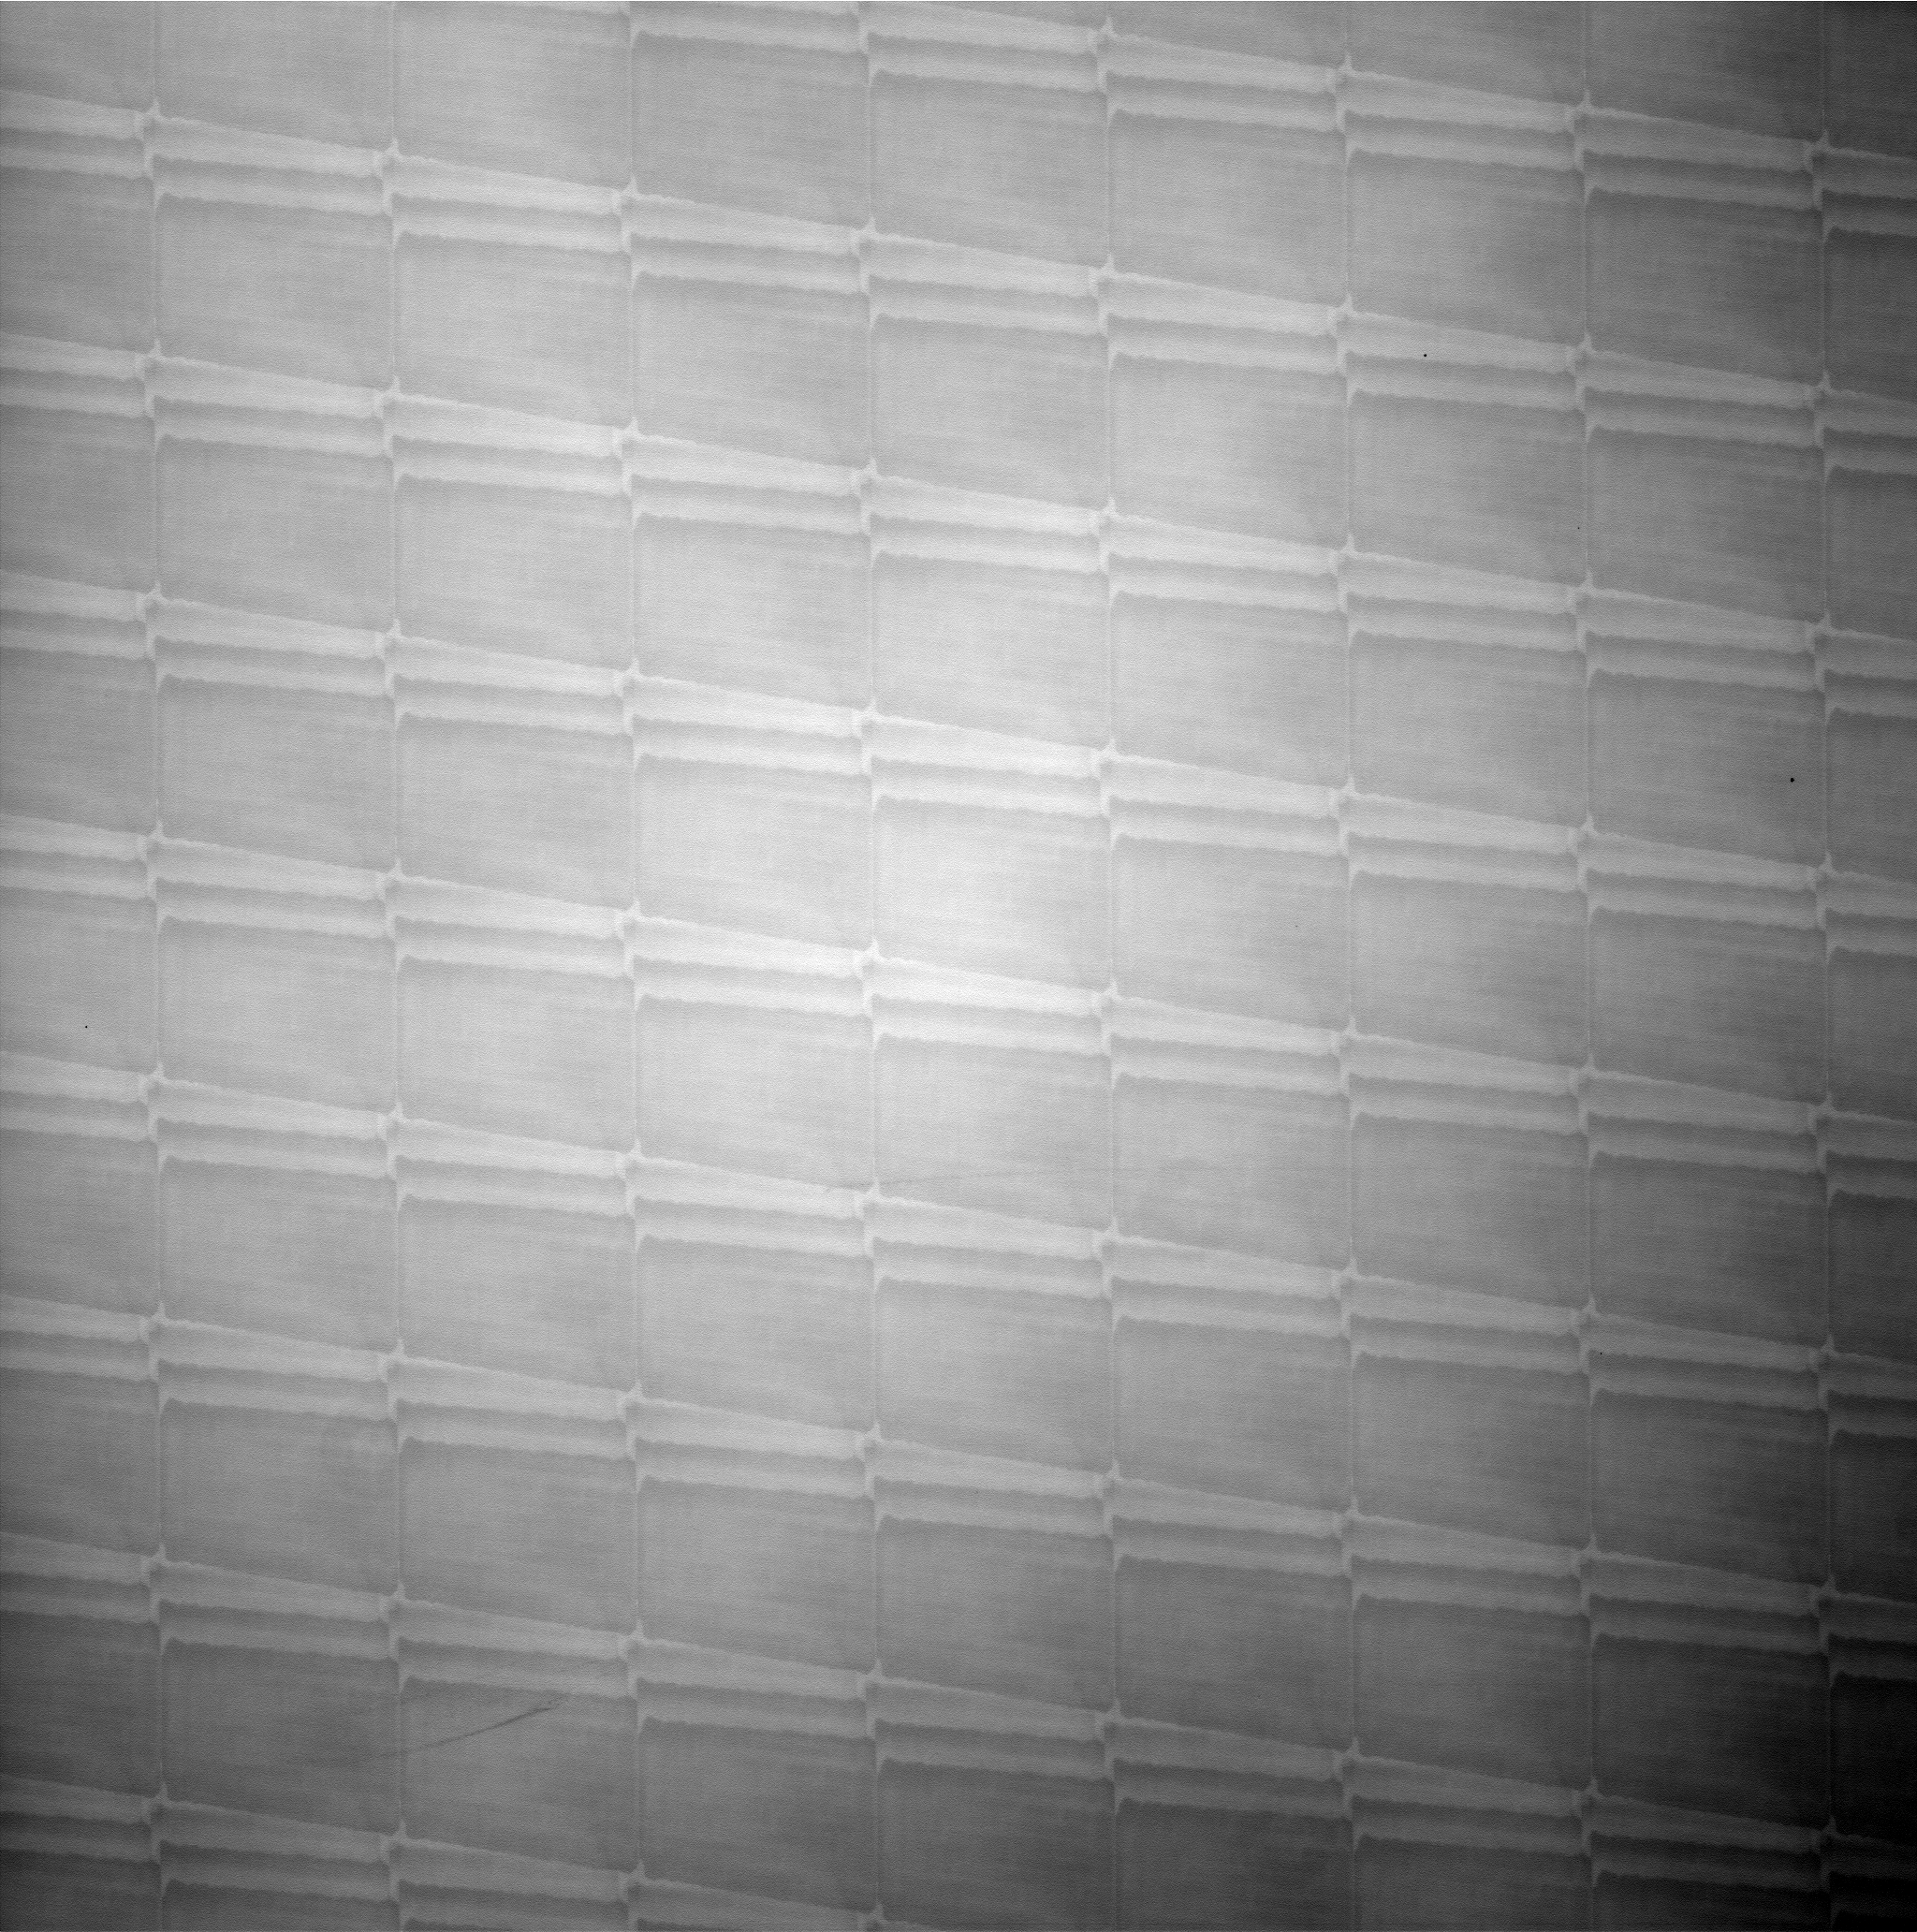
\includegraphics[width=.4\linewidth]{Images/masterflat_OIII.png}}
      \caption{Combined flats for each filter.}
      \label{fig: Masterflats}
    \end{figure}
    
    \begin{figure}[H]
      \centering
      \subfloat[][rSDSS]{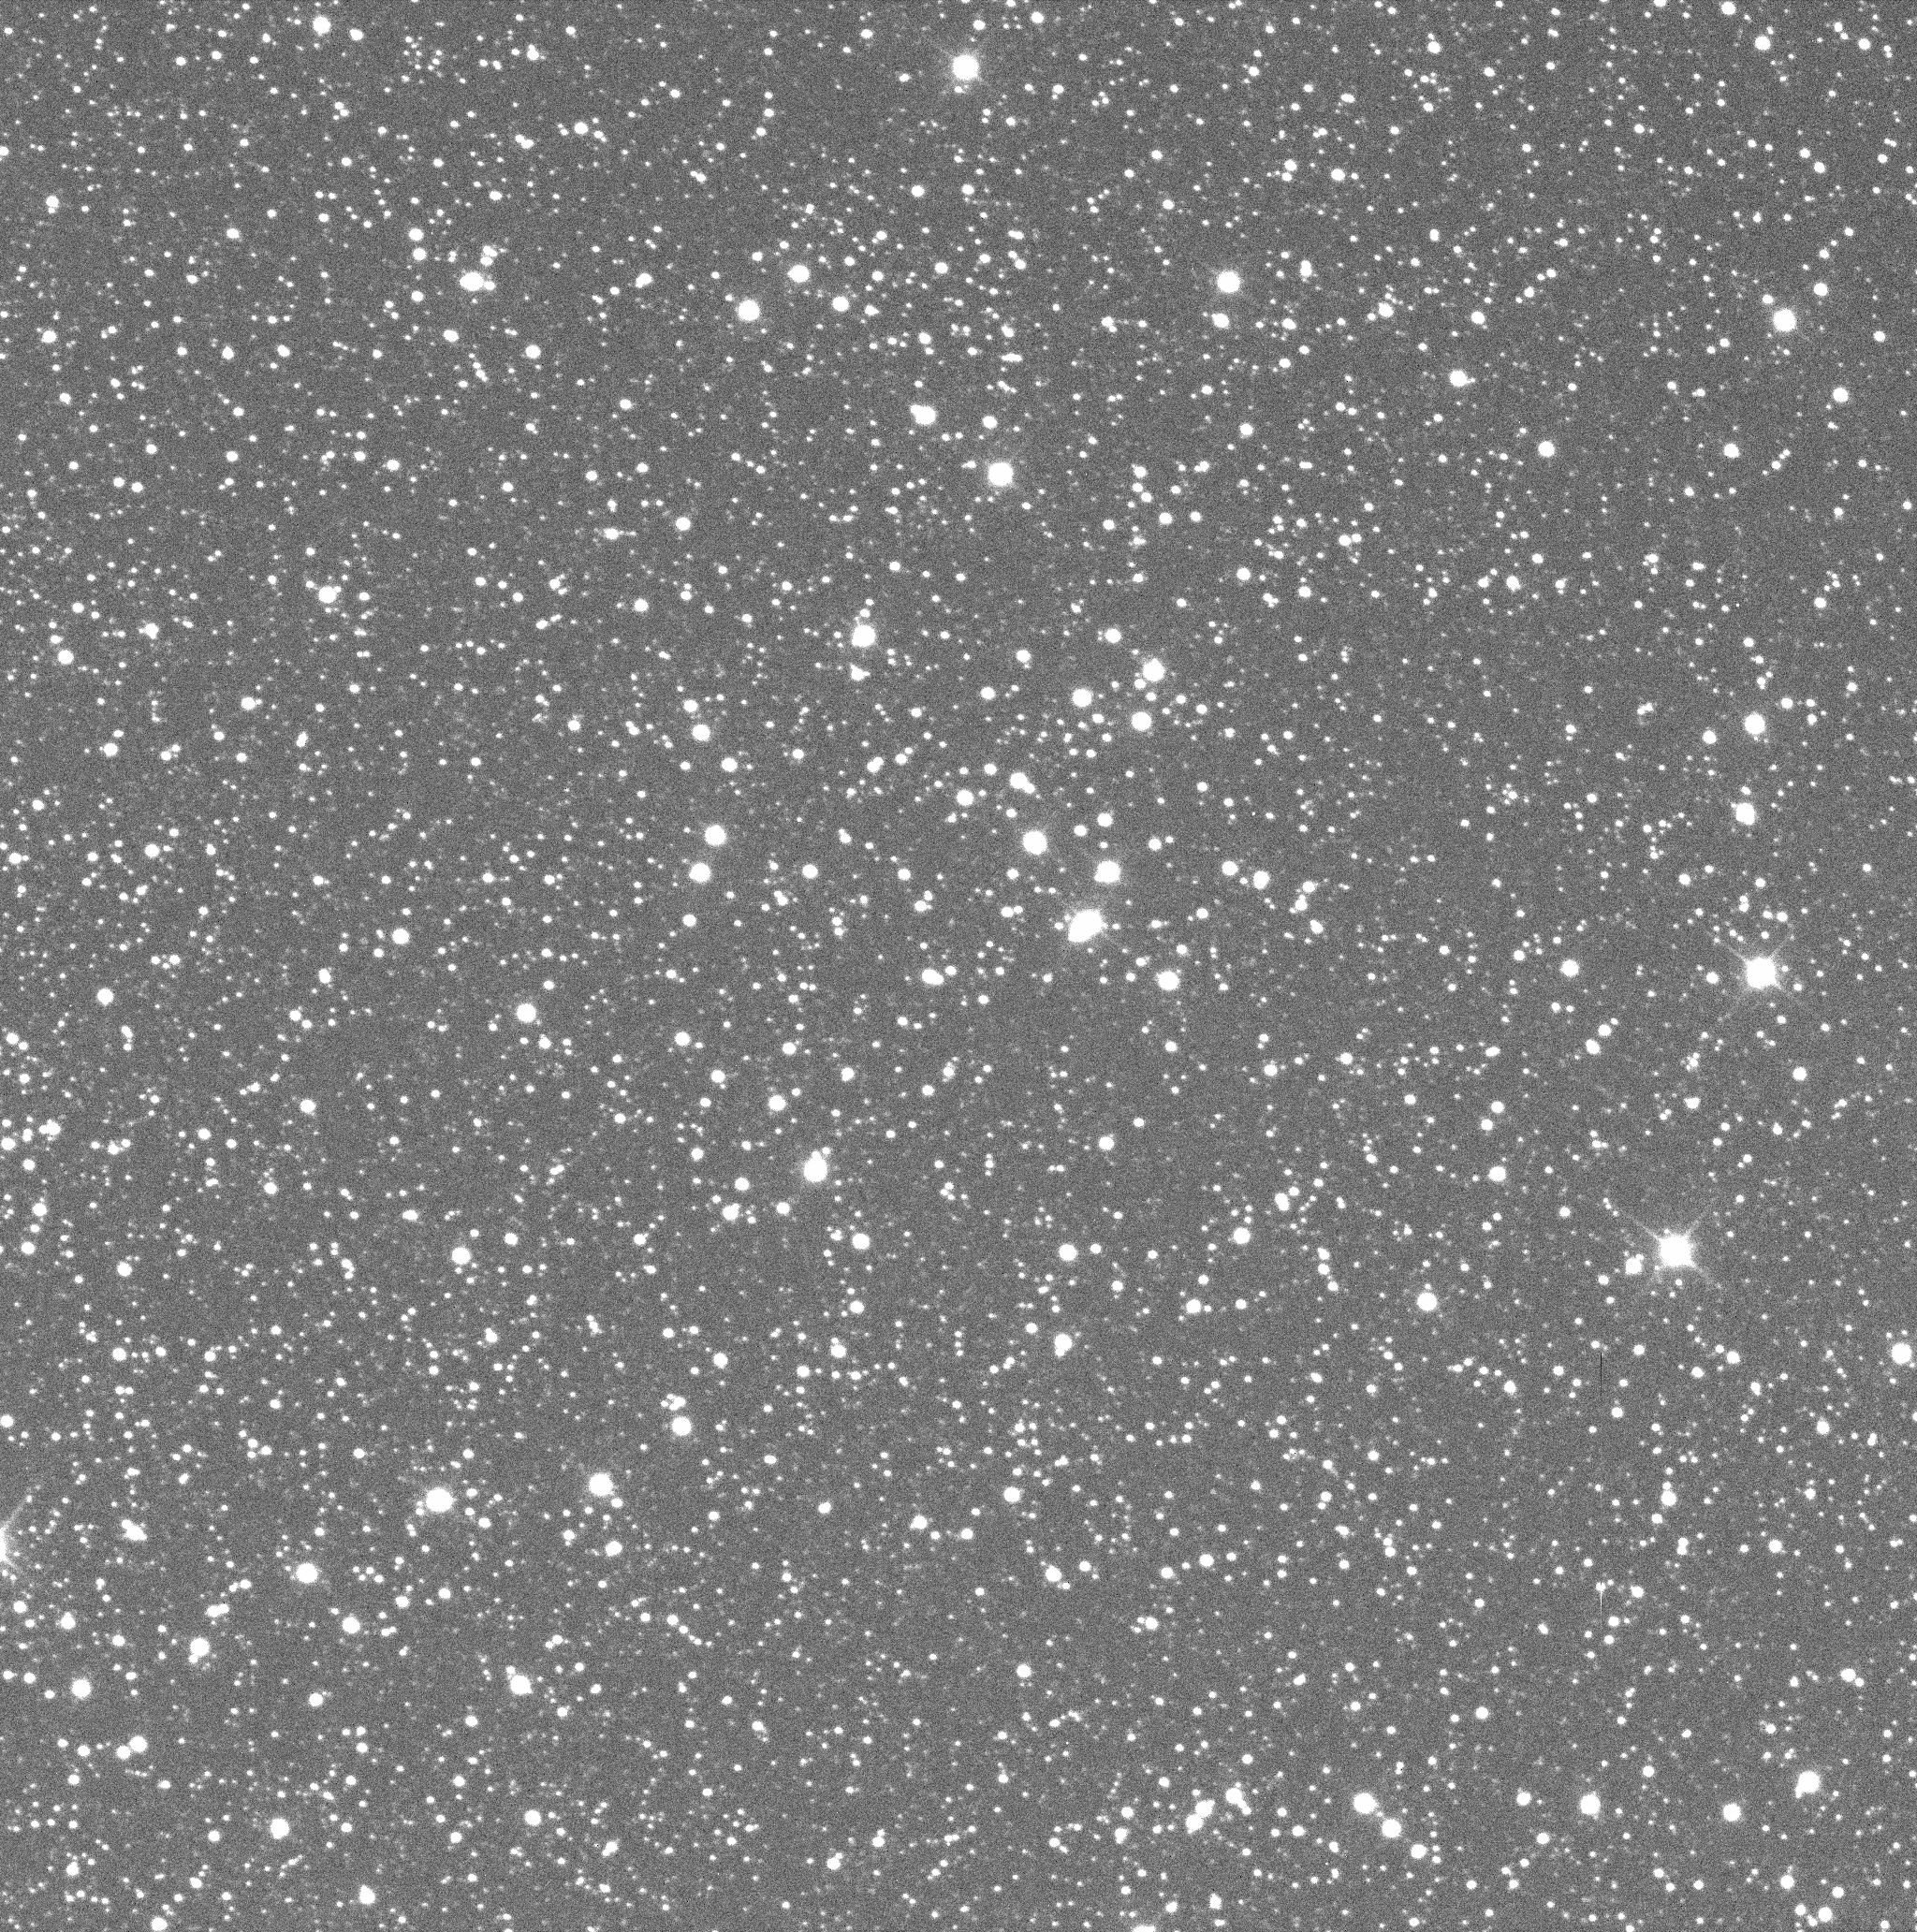
\includegraphics[width=.4\linewidth]{Images/rSDSS.png}}\quad
      \subfloat[][gSDSS]{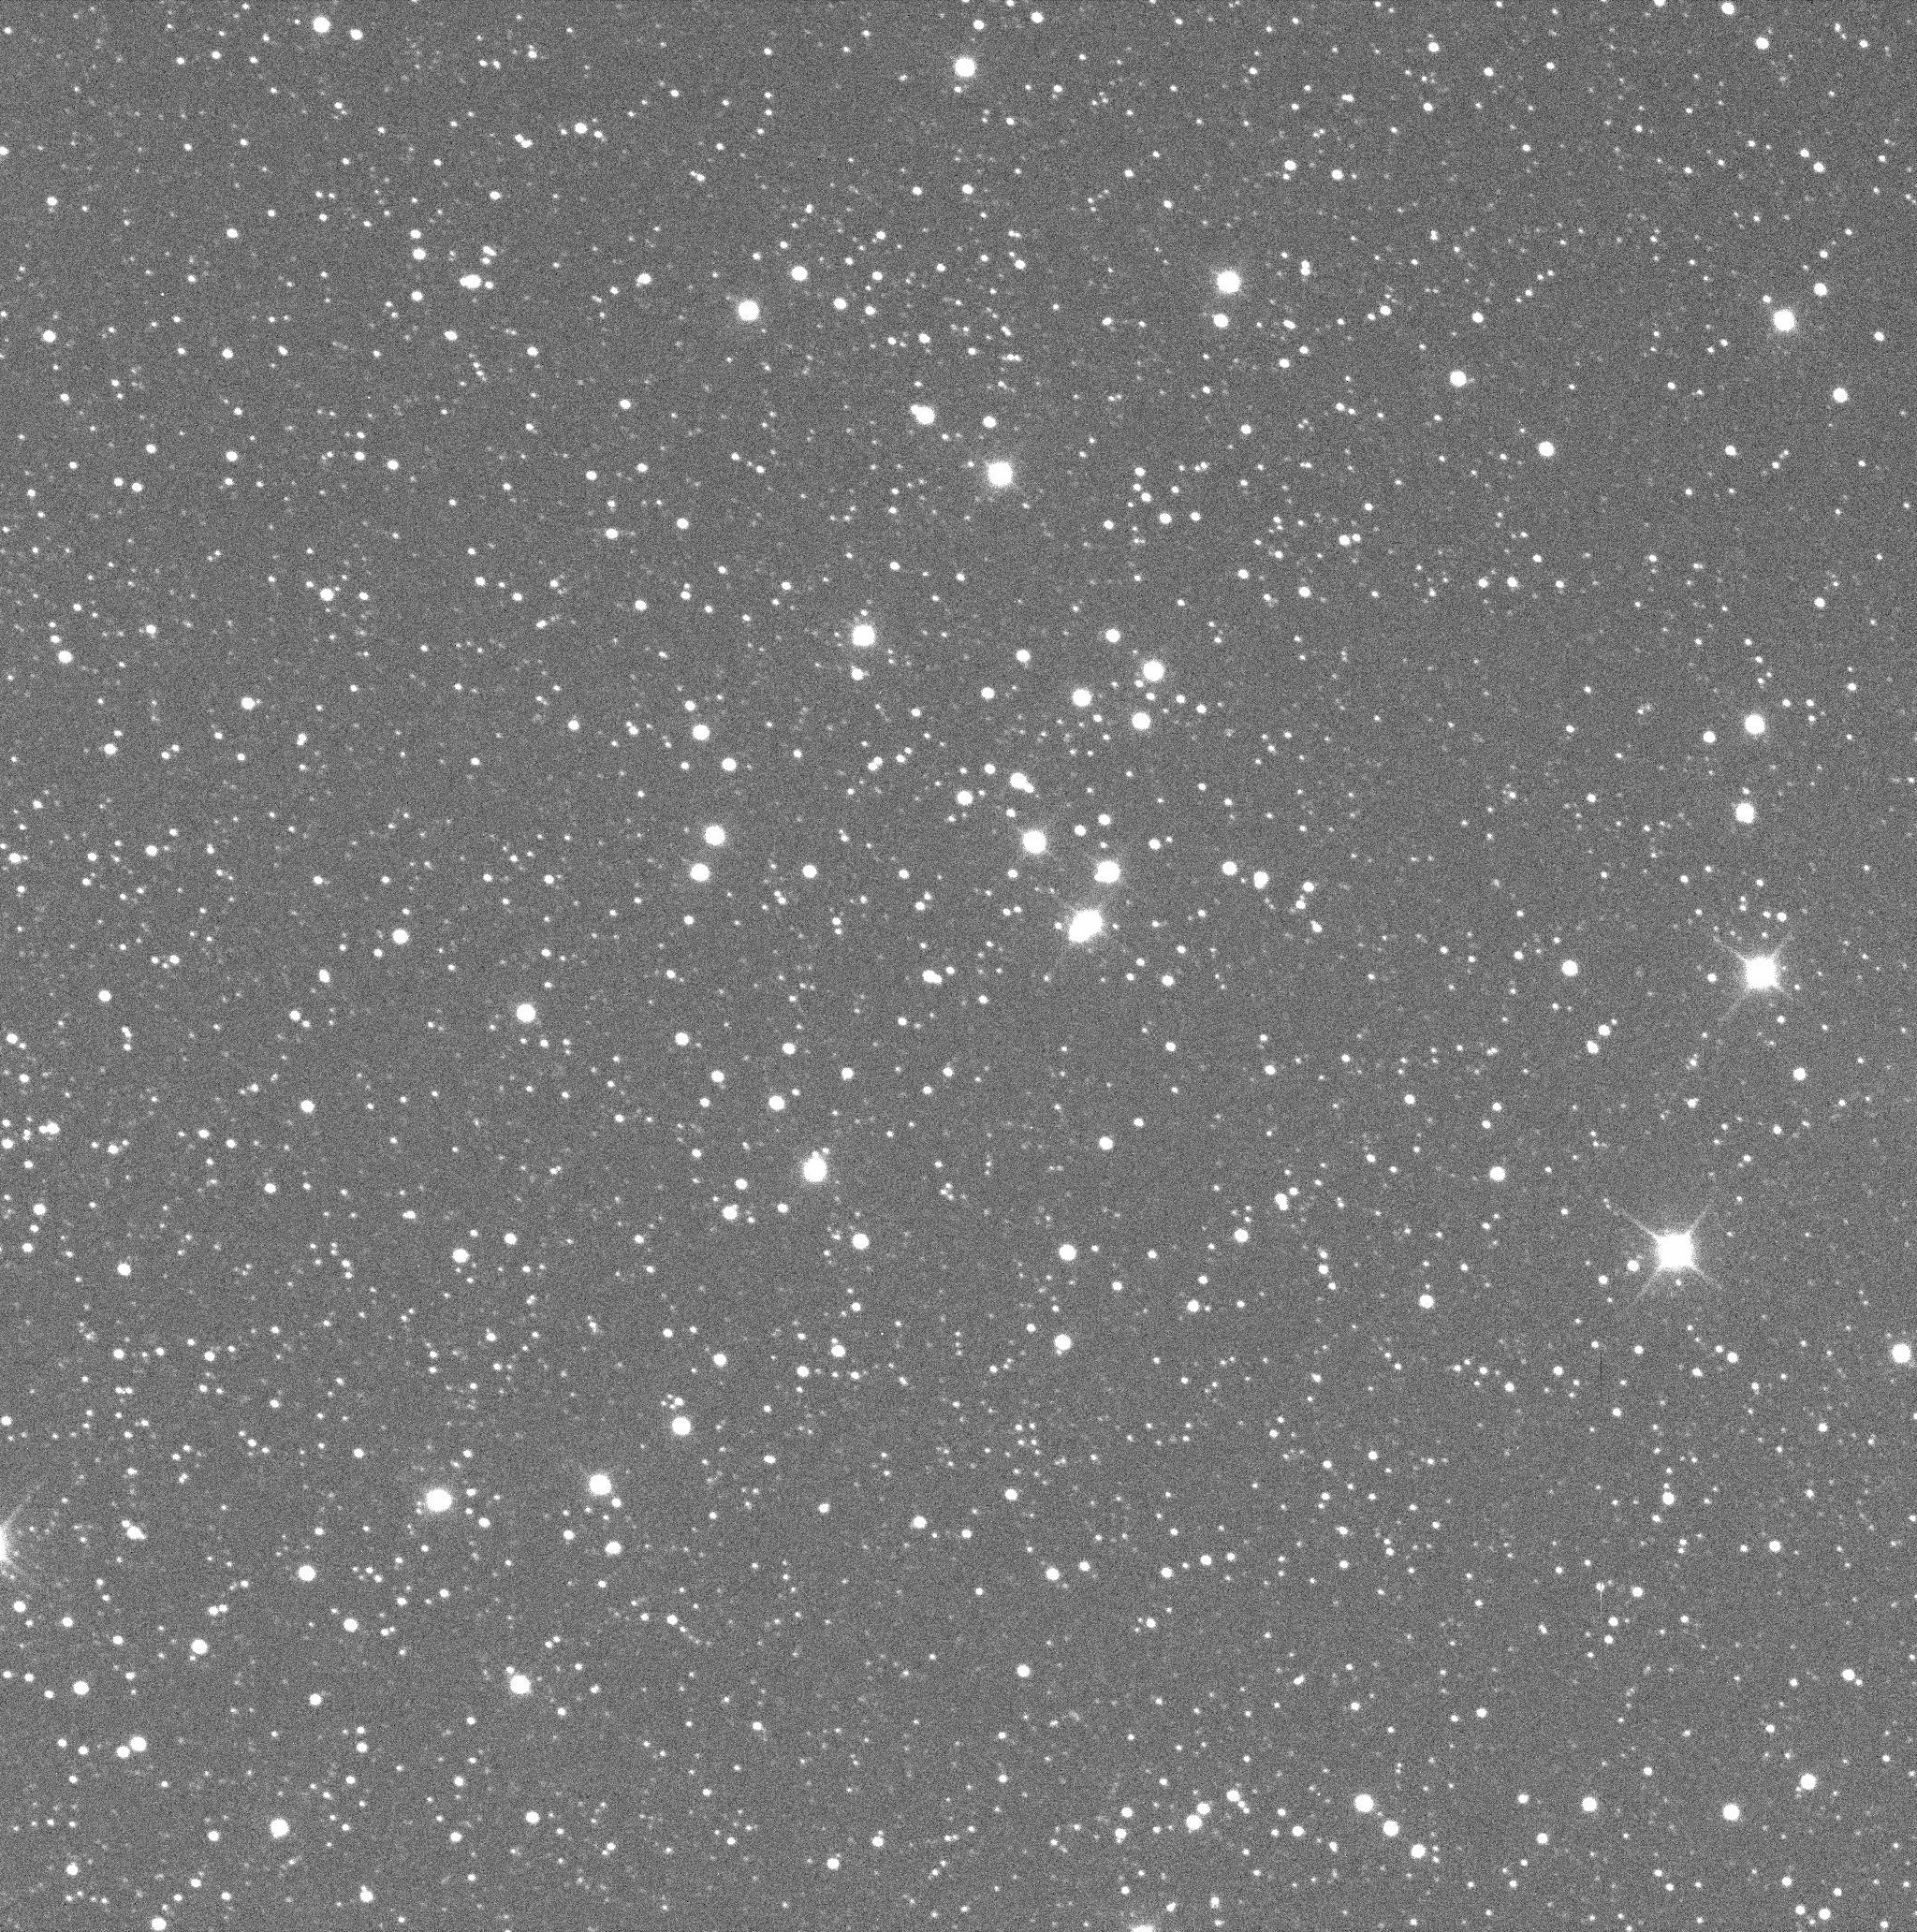
\includegraphics[width=.4\linewidth]{Images/gSDSS.png}}\\
      \subfloat[][Ha]{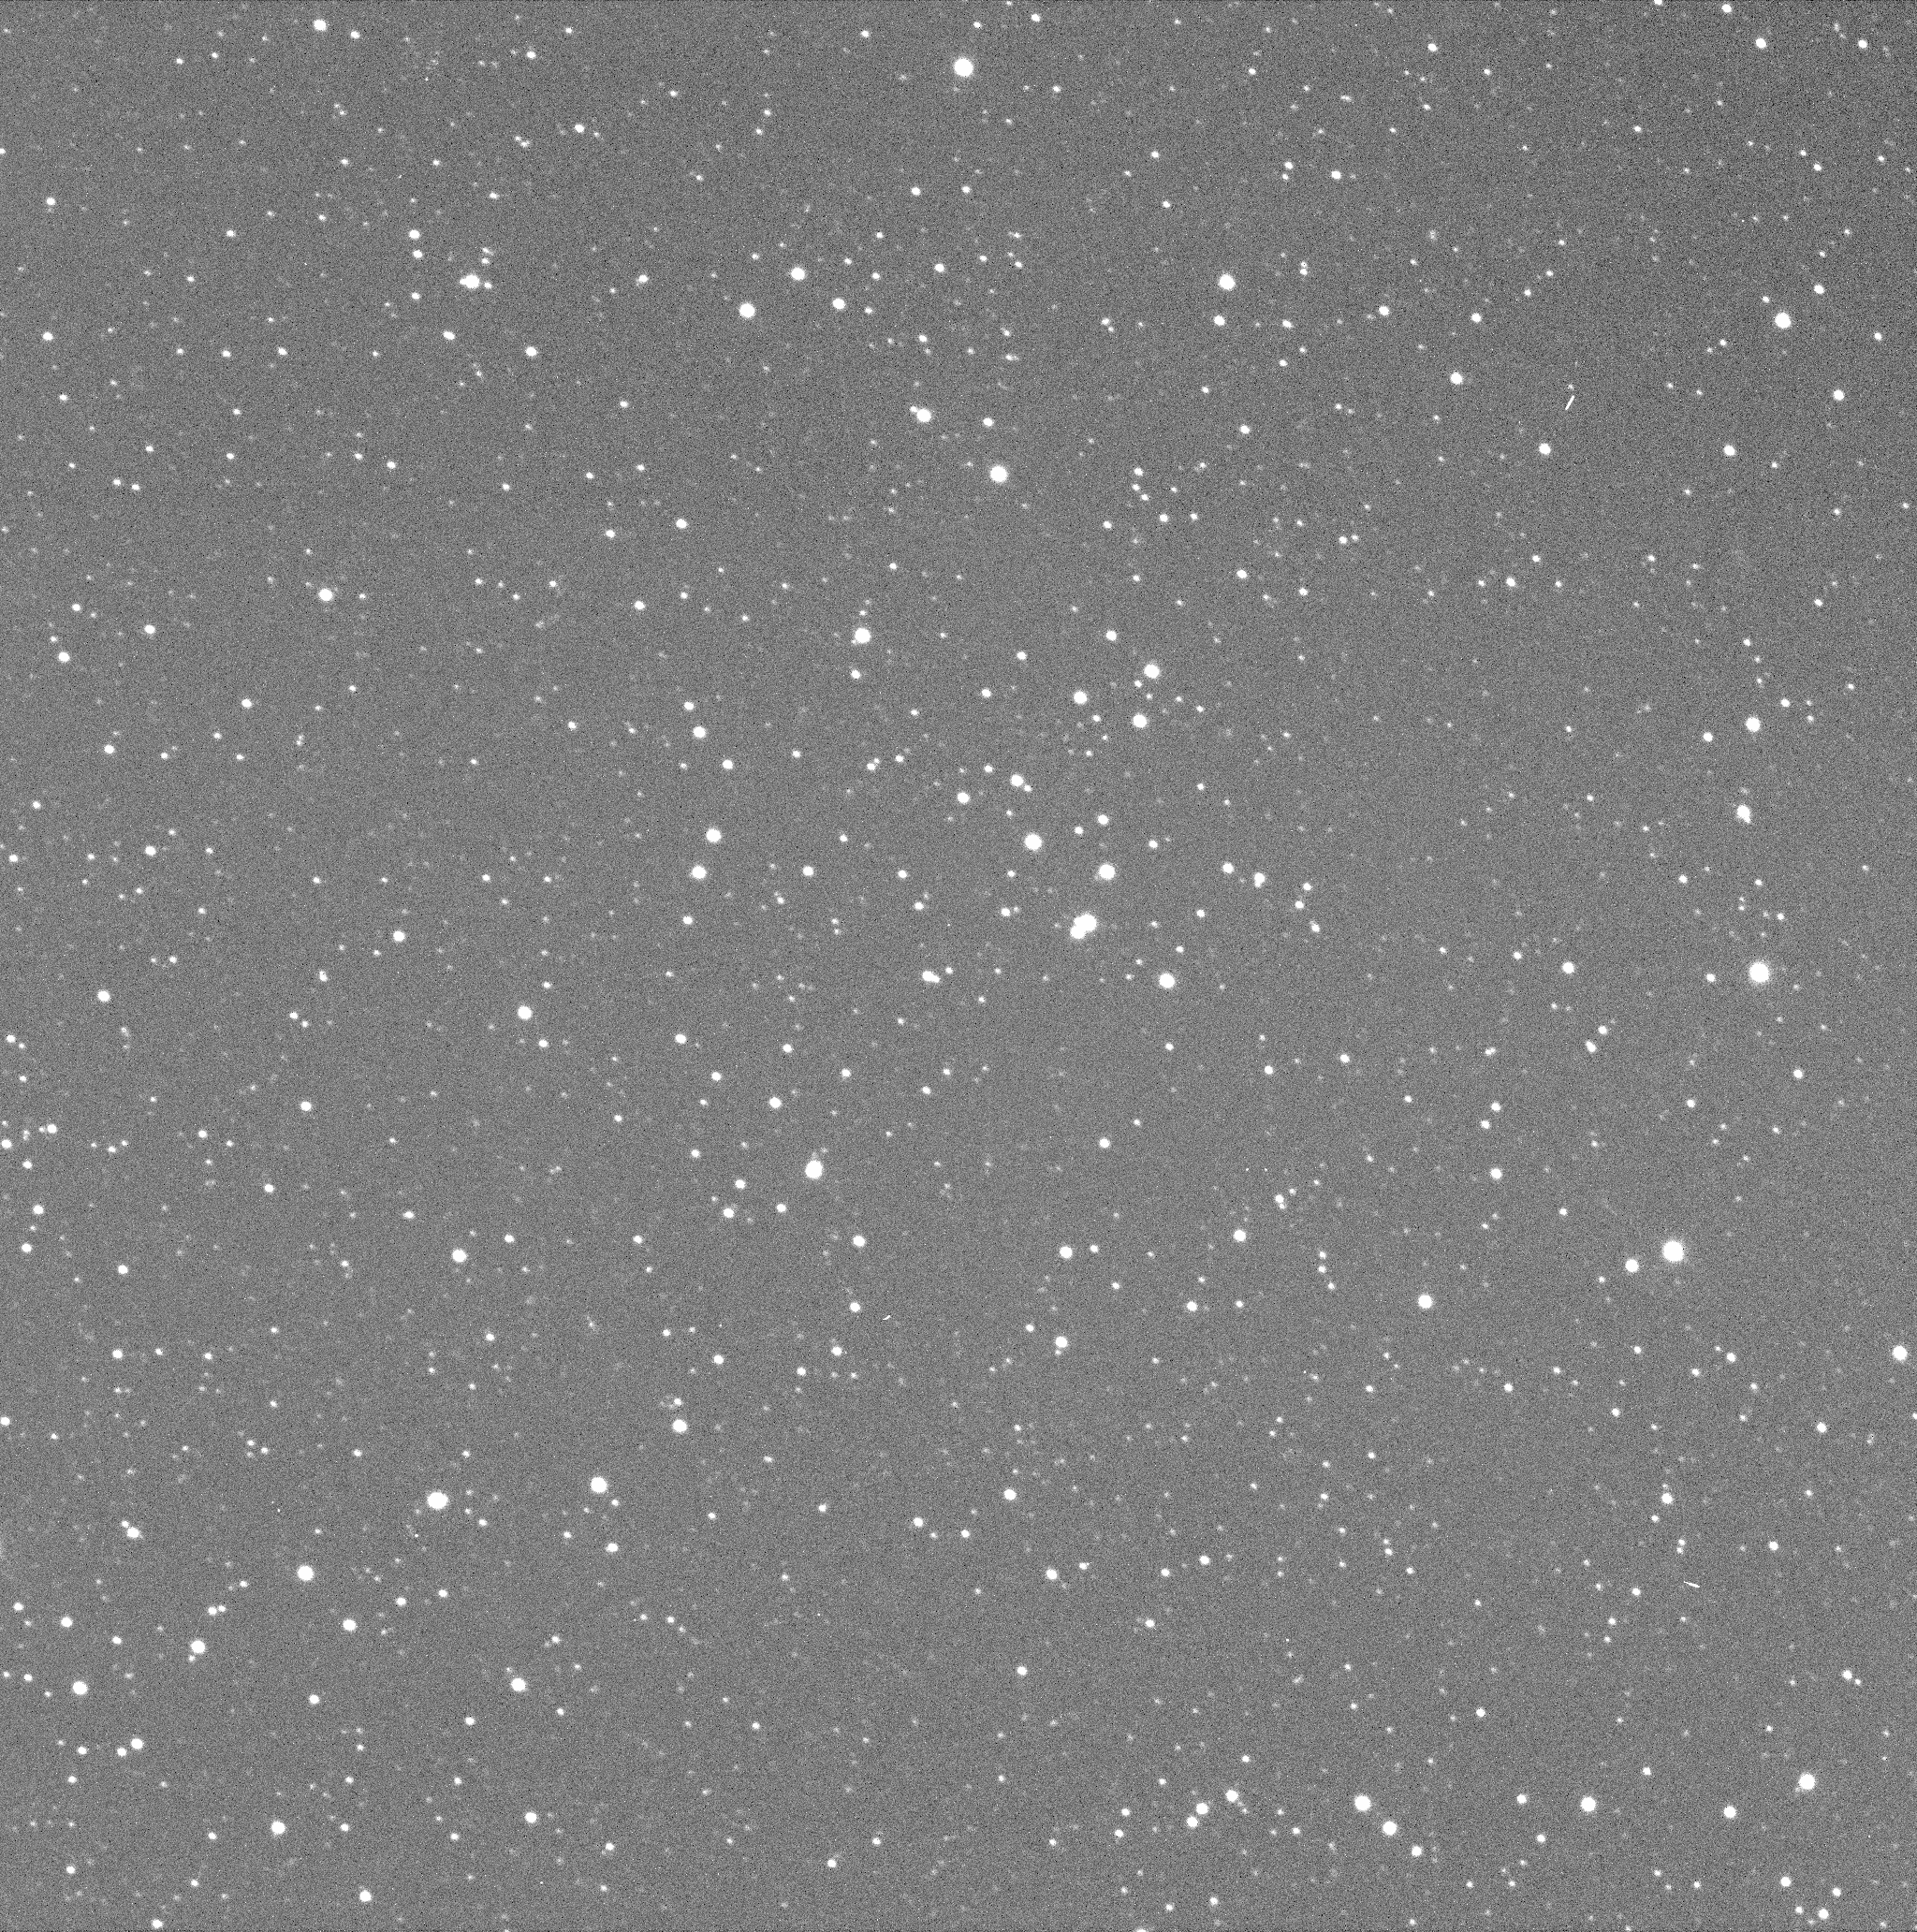
\includegraphics[width=.4\linewidth]{Images/Ha.png}}\quad
      \subfloat[][OIII]{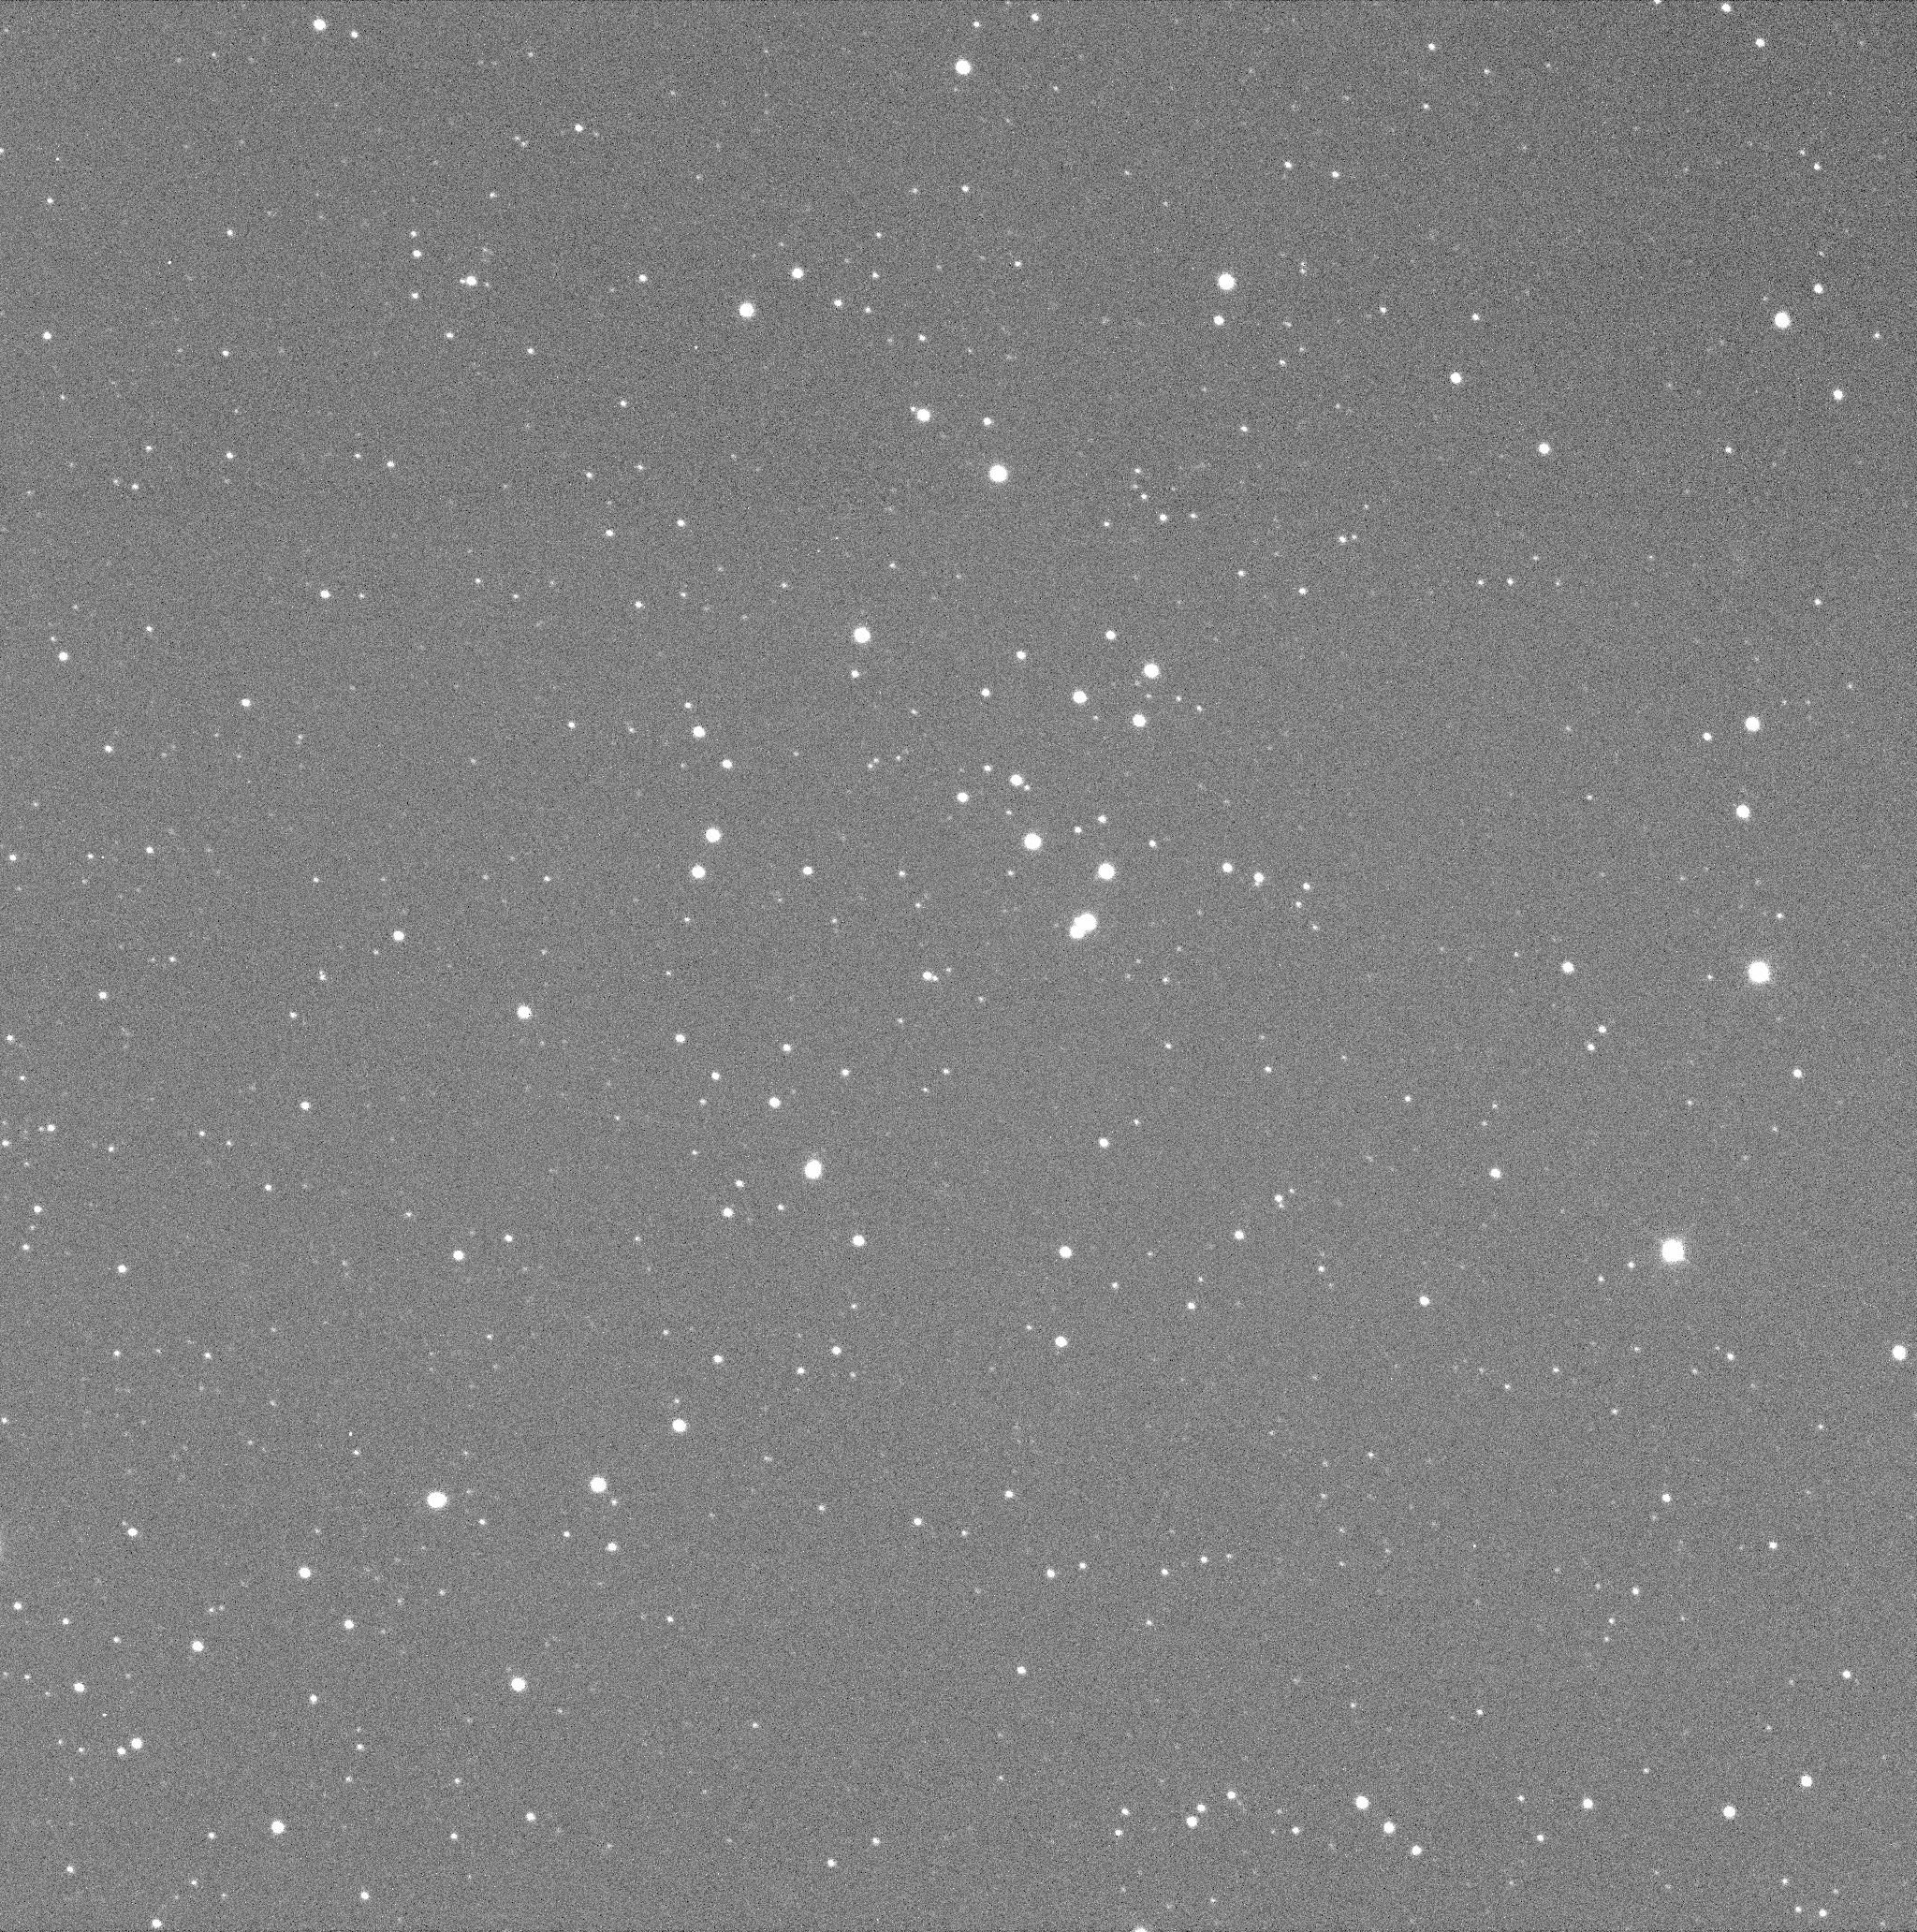
\includegraphics[width=.4\linewidth]{Images/OIII.png}}
      \caption{Reduced scientific images for each filter.}
      \label{fig: Reduced Images}
    \end{figure}

    %%%%%%%%%%%%%%%%%%%%%%%%%%%%%%%%%%%%%%%%%%%%%%%%%%%%%%%%%%%%%%%%%%%%%%%%%%%%%%%%%%%%%%%
    \section{Photometric catalogs}\label{sec: Photometric catalogs}
    %%%%%%%%%%%%%%%%%%%%%%%%%%%%%%%%%%%%%%%%%%%%%%%%%%%%%%%%%%%%%%%%%%%%%%%%%%%%%%%%%%%%%%%
    \section{Some results obtained from the catalogs}\label{sec: Results}
    %%%%%%%%%%%%%%%%%%%%%%%%%%%%%%%%%%%%%%%%%%%%%%%%%%%%%%%%%%%%%%%%%%%%%%%%%%%%%%%%%%%%%%%
    \section{Conclusion}\label{sec: Conclusion}
    
   Sextractor: use "two image mode" first image, must be the "detection" one (the image with better detection range and bigger number of stars) and the second one, the measurement

  \url{ https://nova.astrometry.net/} to calibrate NGC\_6793\_rSDSS.fits

%
%-------------------------------------------------------------------
\nocite{*}
\bibliographystyle{aa}
\bibliography{Biblio}

\end{document}